% Báo cáo giữa kỳ – Quản lý dự án HTTT
% Biên dịch bằng XeLaTeX + Biber (Overleaf: Menu -> Compiler -> XeLaTeX)
\documentclass[a4paper,oneside]{report}
\usepackage[fontsize=13pt]{scrextend}  % cỡ chữ 13pt theo mẫu KLTN

% ---------- Ngôn ngữ, phông chữ ----------
\usepackage{fontspec}
\setmainfont{TeX Gyre Termes}          % tương đương Times New Roman, đủ dấu tiếng Việt
\usepackage[vietnamese]{babel}

% ---------- Trình bày trang ----------
\usepackage[left=3.5cm,right=2cm,top=2.5cm,bottom=2.5cm]{geometry}
\usepackage{setspace}
\onehalfspacing
\setlength{\parindent}{1cm}
\setlength{\parskip}{6pt}
\usepackage{indentfirst}

% ---------- Toán, bảng, hình ----------
\usepackage{amsmath,amssymb}
\numberwithin{equation}{chapter}       % công thức đánh số (1.1), (1.2)... ở lề phải
\usepackage{graphicx}
\graphicspath{{hinh/}{../results/figures/}}
\usepackage{booktabs,longtable,tabularx,multirow,array}
\usepackage{float}
\usepackage[font=small,labelfont=bf]{caption}
\usepackage{xcolor}
\usepackage{enumitem}
\setlist{nosep,leftmargin=1.2cm}

% ---------- Tiêu đề chương ----------
\usepackage{titlesec}
\titleformat{\chapter}[display]{\centering\bfseries\Large}{CHƯƠNG \thechapter}{6pt}{\MakeUppercase}
\titlespacing*{\chapter}{0pt}{0pt}{18pt}
\titleformat{\section}{\bfseries\large}{\thesection}{0.6em}{}
\titleformat{\subsection}{\bfseries\itshape}{\thesubsection}{0.6em}{}

% ---------- Tài liệu tham khảo ----------
\usepackage[backend=biber,style=numeric,sorting=none,maxbibnames=6]{biblatex}
\addbibresource{refs.bib}

\usepackage[hidelinks]{hyperref}

% ---------- Thông tin sinh viên (sửa ở đây) ----------
\newcommand{\truongdh}{TRƯỜNG ĐẠI HỌC ...}
\newcommand{\khoa}{KHOA ...}
\newcommand{\hoten}{Họ và tên sinh viên}
\newcommand{\mssv}{MSSV}
\newcommand{\lop}{Lớp}
\newcommand{\giangvien}{Giảng viên hướng dẫn}
\newcommand{\tende}{QUẢN LÝ RỦI RO TRONG DỰ ÁN XÂY DỰNG DẦU KHÍ\\BẰNG MÔ HÌNH PHƯƠNG TRÌNH CẤU TRÚC PLS-SEM}

\begin{document}

\begin{titlepage}
\begin{center}
{\large\bfseries \truongdh}\\[2pt]
{\large\bfseries \khoa}\\[4pt]
\rule{0.4\textwidth}{0.6pt}\\[3cm]

{\large \hoten}\\[2cm]

{\LARGE\bfseries \tende}\\[2cm]

{\large\bfseries BÁO CÁO GIỮA KỲ}\\[4pt]
{\large Môn học: Quản lý dự án hệ thống thông tin}\\[3cm]

\begin{tabular}{ll}
Mã số sinh viên: & \mssv \\
Lớp: & \lop \\
Giảng viên: & \giangvien \\
\end{tabular}

\vfill
{\large\bfseries HÀ NỘI -- 2026}
\end{center}
\end{titlepage}


\pagenumbering{roman}
\chapter*{Tóm tắt}
\addcontentsline{toc}{chapter}{Tóm tắt}

Báo cáo tìm hiểu bài báo của Kassem (2022) về đánh giá quản lý rủi ro trong dự án xây dựng dầu khí bằng mô hình phương trình cấu trúc bình phương tối thiểu riêng phần (PLS-SEM). Bài báo dùng dữ liệu khảo sát 314 người ở Yemen, xếp hạng 51 yếu tố rủi ro bằng chỉ số tầm quan trọng tương đối (RII) và ma trận xác suất -- tác động, rồi xây dựng mô hình hai bậc đo ảnh hưởng của rủi ro nội bộ và rủi ro bên ngoài tới thành công dự án.

Báo cáo trình bày cơ sở lý thuyết về quản lý rủi ro theo PMBOK và ISO~31000, cùng công thức và cách hoạt động của từng phương pháp. Vì dữ liệu gốc không được công bố, báo cáo tái hiện thực nghiệm theo hai hướng: kiểm tra tính nhất quán của số liệu đã công bố, và chạy lại toàn bộ quy trình trên một bộ dữ liệu mô phỏng có cấu trúc giống bài báo, với thuật toán PLS-SEM tự cài đặt bằng Python. Kết quả cho thấy phần tính toán cơ bản và kết luận chính của bài báo (rủi ro bên ngoài mạnh hơn rủi ro nội bộ) tái hiện được. Tuy nhiên, giá trị phân biệt không đạt ở một số nhóm rủi ro, và hệ số của 13 giả thuyết chi tiết không tái hiện được. Hai ví dụ thực tế, gồm dự án Nhiệt điện Thái Bình 2 và dự án Healthcare.gov, cùng phần minh họa bằng MS Project, Excel và mô phỏng Monte Carlo, cho thấy khung rủi ro của bài báo dùng lại được, nhưng mức độ quan trọng của từng nhóm rủi ro phụ thuộc mạnh vào bối cảnh.

\textbf{Từ khóa:} quản lý rủi ro, dự án xây dựng dầu khí, RII, ma trận xác suất -- tác động, PLS-SEM, HTMT, Monte Carlo.

\clearpage


\tableofcontents
\clearpage
\chapter*{Danh sách thuật ngữ và từ viết tắt}
\addcontentsline{toc}{chapter}{Danh sách thuật ngữ và từ viết tắt}

\begin{longtable}{@{}p{2.2cm}p{5.6cm}p{6.2cm}@{}}
\toprule
\textbf{Viết tắt} & \textbf{Tiếng Anh} & \textbf{Tiếng Việt} \\
\midrule
\endhead
AVE & Average Variance Extracted & Phương sai trung bình được trích \\
CB-SEM & Covariance-Based SEM & SEM dựa trên hiệp phương sai \\
CR & Composite Reliability & Độ tin cậy tổng hợp \\
GoF & Goodness of Fit & Độ phù hợp của mô hình \\
HTMT & Heterotrait--Monotrait ratio & Tỷ số dị biệt -- đơn biệt \\
PIM & Probability--Impact Matrix & Ma trận xác suất -- tác động \\
PLS-SEM & Partial Least Squares SEM & Mô hình cấu trúc bình phương tối thiểu riêng phần \\
PMBOK & Project Management Body of Knowledge & Bộ kiến thức quản lý dự án \\
RII & Relative Importance Index & Chỉ số tầm quan trọng tương đối \\
SEM & Structural Equation Modeling & Mô hình phương trình cấu trúc \\
\bottomrule
\end{longtable}

\clearpage

\listoffigures
\clearpage
\listoftables
\clearpage

\pagenumbering{arabic}
\chapter*{Mở đầu}
\addcontentsline{toc}{chapter}{Mở đầu}

% Viết ngày 02/11, khoảng 1 trang:
% - Lý do chọn đề tài: dự án xây dựng hay vượt chi phí, trễ tiến độ; quản lý rủi ro là một vùng kiến thức của PMBOK.
% - Bài báo được nghiên cứu: Kassem (2022).
% - Mục tiêu báo cáo: (1) hiểu và trình bày phương pháp; (2) tái hiện phân tích; (3) liên hệ thực tế.
% - Bố cục 4 chương.

\chapter{Tổng quan về quản lý rủi ro dự án}
\label{chuong:tong-quan}

Chương này trình bày các khái niệm nền tảng để đọc hiểu bài báo của Kassem~\cite{kassem2022}: dự án và thước đo thành công của dự án, khái niệm rủi ro và quy trình quản lý rủi ro theo PMBOK và ISO~31000, đặc thù của dự án xây dựng trong ngành dầu khí, và các kỹ thuật quản lý rủi ro thường dùng.

\section{Dự án và thành công của dự án}
\label{sec:du-an}

Theo PMBOK~\cite{pmbok6}, dự án là \emph{một nỗ lực tạm thời nhằm tạo ra một sản phẩm, dịch vụ hoặc kết quả duy nhất}. Hai đặc điểm ``tạm thời'' và ``duy nhất'' cũng là nguồn gốc của rủi ro: dự án nào cũng có điểm mới, chưa từng làm đúng y như vậy, nên kinh nghiệm từ dự án trước chỉ dùng được một phần.

Thành công của dự án từ lâu được đo bằng ba tiêu chí \textbf{thời gian, chi phí và chất lượng}, thường gọi là ``tam giác sắt''. Atkinson~\cite{atkinson1999} cho rằng ba tiêu chí này chỉ là ``hai phỏng đoán và một hiện tượng'': thời gian và chi phí được ước tính từ khi chưa có đủ thông tin, còn chất lượng là khái niệm thay đổi theo người đánh giá. Vì vậy ông đề xuất bổ sung các tiêu chí như lợi ích cho tổ chức và cho các bên liên quan. Bài báo của Kassem vẫn đi theo cách tiếp cận truyền thống: thành công được đo ngược lại qua năm hậu quả xấu là trễ tiến độ, vượt chi phí, chất lượng kém, không đạt mục tiêu và dự án bị dừng~\cite{kassem2022}.

Trong ngành xây dựng, vượt chi phí và trễ tiến độ là hiện tượng phổ biến. Ở các nước kém phát triển, mức vượt có khi hơn 100\% so với kế hoạch~\cite{kassem2022}. Nguyên nhân thường được nhắc tới là các bên tham gia không nhận diện và kiểm soát được rủi ro ngay từ đầu dự án.

\section{Rủi ro và quản lý rủi ro}
\label{sec:rui-ro}

\subsection{Khái niệm rủi ro}

PMBOK~\cite{pmbok6} định nghĩa rủi ro dự án riêng lẻ là \emph{một sự kiện hoặc điều kiện không chắc chắn, nếu xảy ra sẽ gây tác động tích cực hoặc tiêu cực tới một hay nhiều mục tiêu của dự án}. Tiêu chuẩn ISO~31000:2018~\cite{iso31000} định nghĩa ngắn gọn hơn: rủi ro là \emph{ảnh hưởng của sự không chắc chắn lên mục tiêu}.

Hai định nghĩa có ba điểm chung đáng chú ý:
\begin{itemize}
  \item Rủi ro gắn với \textbf{mục tiêu}. Không có mục tiêu thì không có rủi ro.
  \item Rủi ro có hai chiều: \textbf{khả năng xảy ra} (xác suất) và \textbf{mức ảnh hưởng} (tác động). Đây chính là hai trục của ma trận xác suất -- tác động và là hai thành phần của chỉ số RII trình bày ở Chương~\ref{chuong:phuong-phap}.
  \item Rủi ro có thể là \textbf{mối đe dọa} (tác động tiêu cực) hoặc \textbf{cơ hội} (tác động tích cực). Bài báo của Kassem chỉ xét mặt tiêu cực.
\end{itemize}

\subsection{Quy trình quản lý rủi ro theo PMBOK}

PMBOK phiên bản 6~\cite{pmbok6} coi quản lý rủi ro là một trong mười vùng kiến thức và chia thành bảy quy trình (Bảng~\ref{tab:quy-trinh-pmbok}).

\begin{table}[H]
\centering
\caption{Bảy quy trình quản lý rủi ro dự án theo PMBOK 6~\cite{pmbok6}}
\label{tab:quy-trinh-pmbok}
\begin{tabularx}{\textwidth}{@{}clX@{}}
\toprule
\textbf{TT} & \textbf{Quy trình} & \textbf{Nội dung chính} \\
\midrule
1 & Lập kế hoạch quản lý rủi ro & Xác định cách thức tiến hành quản lý rủi ro cho dự án \\
2 & Nhận diện rủi ro & Lập danh sách rủi ro, nguồn gốc và đặc điểm của chúng (sổ đăng ký rủi ro) \\
3 & Phân tích định tính & Xếp ưu tiên rủi ro theo xác suất và tác động \\
4 & Phân tích định lượng & Ước lượng bằng số ảnh hưởng tổng hợp của rủi ro lên mục tiêu dự án \\
5 & Lập kế hoạch ứng phó & Chọn chiến lược và hành động xử lý từng rủi ro \\
6 & Thực hiện ứng phó & Triển khai các hành động đã thống nhất \\
7 & Giám sát rủi ro & Theo dõi rủi ro đã biết, phát hiện rủi ro mới, đánh giá hiệu quả ứng phó \\
\bottomrule
\end{tabularx}
\end{table}

Với các mối đe dọa, PMBOK đưa ra năm chiến lược ứng phó: \textbf{báo cáo lên cấp trên} khi rủi ro vượt thẩm quyền của dự án, \textbf{né tránh}, \textbf{chuyển giao} (ví dụ mua bảo hiểm hoặc đưa vào hợp đồng), \textbf{giảm thiểu} và \textbf{chấp nhận}.

PMBOK phiên bản 7~\cite{pmbok7} chuyển từ cách tiếp cận theo quy trình sang cách tiếp cận theo nguyên tắc và miền hiệu suất. Quản lý rủi ro nằm trong miền hiệu suất \emph{Sự không chắc chắn} (Uncertainty) và nguyên tắc \emph{Tối ưu hóa ứng phó rủi ro}. Tuy vậy, các công cụ như sổ đăng ký rủi ro hay ma trận xác suất -- tác động vẫn được giữ nguyên.

\subsection{Quy trình quản lý rủi ro theo ISO 31000}

ISO~31000:2018~\cite{iso31000} là tiêu chuẩn chung cho mọi loại tổ chức, không riêng cho dự án. Quy trình gồm: thiết lập phạm vi, bối cảnh và tiêu chí; \textbf{đánh giá rủi ro} (gồm nhận diện, phân tích và định mức rủi ro); xử lý rủi ro; giám sát và xem xét. Song song với đó là trao đổi, tham vấn, ghi nhận và báo cáo xuyên suốt cả quá trình.

So sánh hai cách tiếp cận: bước ``đánh giá rủi ro'' của ISO~31000 tương ứng với ba quy trình 2, 3, 4 của PMBOK. Nghiên cứu của Kassem nằm trọn trong bước này. Bài báo nhận diện 51 yếu tố rủi ro, phân tích định tính bằng RII và ma trận xác suất -- tác động, rồi dùng mô hình PLS-SEM để định lượng mức ảnh hưởng của từng nhóm rủi ro lên thành công dự án. Phần ứng phó chỉ dừng ở các khuyến nghị chung cho từng bên liên quan.

\section{Đặc thù của dự án xây dựng dầu khí}
\label{sec:dau-khi}

Dự án xây dựng trong ngành dầu khí (nhà máy xử lý, đường ống, kho bể, cơ sở hạ tầng mỏ) có rủi ro cao hơn dự án xây dựng thông thường vì một số lý do~\cite{kassem2022,thuyet2007}:
\begin{itemize}
  \item \textbf{Vốn đầu tư lớn}, nên một tỷ lệ vượt chi phí nhỏ cũng là con số tuyệt đối rất lớn.
  \item \textbf{Nhiều bên tham gia}: chủ đầu tư thường là nhà nước hoặc công ty dầu khí quốc gia, cùng với nhà thầu EPC, nhà thầu phụ, tư vấn và nhà cung cấp quốc tế.
  \item \textbf{Công nghệ phức tạp}, thiết bị phải nhập khẩu, dễ chịu ảnh hưởng của chuỗi cung ứng.
  \item \textbf{Ảnh hưởng lớn tới môi trường và cộng đồng}, nên chịu nhiều ràng buộc pháp lý và sự phản đối của người dân địa phương.
  \item \textbf{Gắn với chính trị và kinh tế vĩ mô}: dầu khí là tài sản quốc gia, nên chịu tác động trực tiếp của chính sách, giá dầu và tình hình an ninh.
\end{itemize}

Bối cảnh của bài báo là Yemen, nơi xảy ra nội chiến từ năm 2015. Theo tác giả, xung đột đã làm dừng phần lớn hoạt động khai thác và dự án dầu khí~\cite{kassem2022}. Đây là yếu tố cần nhớ khi diễn giải kết quả ``rủi ro bên ngoài lấn át rủi ro nội bộ'' ở các chương sau. Nghiên cứu của Thuyet và cộng sự~\cite{thuyet2007} về dự án dầu khí tại Việt Nam là một đối chiếu hữu ích, vì bối cảnh chính trị ổn định hơn nhiều.

\section{Các kỹ thuật quản lý rủi ro}
\label{sec:ky-thuat}

Bài báo liệt kê 22 kỹ thuật quản lý rủi ro hay được dùng trong các nghiên cứu trước (Bảng~1 trong~\cite{kassem2022}), nhưng không phân loại chúng. Bảng~\ref{tab:ky-thuat} sắp xếp lại các kỹ thuật đó theo quy trình PMBOK mà chúng phục vụ chủ yếu. Một số kỹ thuật dùng được ở nhiều bước, ở đây chỉ xếp vào bước điển hình nhất.

\begin{longtable}{@{}p{4.3cm}p{5.3cm}p{4.4cm}@{}}
\caption{Các kỹ thuật quản lý rủi ro trong bài báo, phân theo quy trình PMBOK}
\label{tab:ky-thuat}\\
\toprule
\textbf{Quy trình} & \textbf{Kỹ thuật} & \textbf{Tên tiếng Anh} \\
\midrule
\endfirsthead
\toprule
\textbf{Quy trình} & \textbf{Kỹ thuật} & \textbf{Tên tiếng Anh} \\
\midrule
\endhead
\multirow{10}{4.3cm}{Nhận diện rủi ro}
 & Động não & Brainstorming \\
 & Danh mục kiểm tra & Checklist \\
 & Phỏng vấn & Interviews \\
 & Phương pháp Delphi & Delphi Method \\
 & Ý kiến chuyên gia & Expert Judgement \\
 & Phân tích thay đổi & Change Analysis (ChA) \\
 & Cấu trúc phân rã rủi ro & Risk Breakdown Structure (RBS) \\
 & Ma trận phân rã rủi ro & Risk Breakdown Matrix (RBM) \\
 & Phân tích SWOT & SWOT Analysis \\
 & Rà soát mối nguy & Hazard Review (HR) \\
\midrule
\multirow{8}{4.3cm}{Phân tích định tính}
 & Ma trận xác suất -- tác động & Probability and Impact Matrix \\
 & Chỉ số tầm quan trọng tương đối & Relative Importance Index (RII) \\
 & Chỉ số rủi ro & Risk Index \\
 & Phân tích Pareto & Pareto Analysis (PA) \\
 & Phân tích dạng lỗi và tác động & FMEA \\
 & Phân tích mối nguy và khả năng vận hành & HAZOP \\
 & Phân tích nguyên nhân -- hệ quả & Cause and Consequence Analysis \\
 & Sơ đồ nhân tố nguyên nhân sự kiện & Event Causal Factor Charting \\
\midrule
\multirow{4}{4.3cm}{Phân tích định lượng}
 & Mô phỏng Monte Carlo & Monte Carlo Method \\
 & Giá trị tiền tệ kỳ vọng & Expected Monetary Value (EMV) \\
 & Phân tích cây lỗi & Fault Tree Analysis (FTA) \\
 & Logic mờ & Fuzzy Logic \\
\bottomrule
\end{longtable}

Có thể rút ra hai nhận xét từ bảng trên:
\begin{enumerate}
  \item Phần lớn các kỹ thuật thuộc nhóm \textbf{nhận diện} và \textbf{phân tích định tính}. Chúng dựa nhiều vào ý kiến chủ quan của chuyên gia và người tham gia dự án. RII và ma trận xác suất -- tác động mà bài báo sử dụng cũng thuộc nhóm này: đầu vào là điểm số trên thang Likert do người trả lời tự đánh giá.
  \item Bảng không có kỹ thuật nào để đo \textbf{quan hệ nhân quả giữa các nhóm rủi ro và kết quả dự án}. Đây là khoảng trống mà bài báo muốn lấp bằng mô hình phương trình cấu trúc (SEM). SEM không nằm trong bộ công cụ chuẩn của PMBOK mà đến từ thống kê trong khoa học xã hội và quản trị~\cite{hair2022primer}.
\end{enumerate}

\section{Sơ đồ tổng quan chủ đề}
\label{sec:so-do}

% Sơ đồ tư duy: thêm hình hinh/so-do-tu-duy.png

\chapter{Phương pháp và mô hình nghiên cứu}
\label{chuong:phuong-phap}

Bài báo của Kassem~\cite{kassem2022} kết hợp ba lớp phân tích trên cùng một bộ dữ liệu khảo sát 314 phiếu: chỉ số tầm quan trọng tương đối (RII) để xếp hạng từng yếu tố rủi ro, ma trận xác suất -- tác động (PIM) để phân vùng rủi ro, và mô hình phương trình cấu trúc bình phương tối thiểu riêng phần (PLS-SEM) để đo ảnh hưởng của các nhóm rủi ro lên thành công dự án. Chương này trình bày cơ sở lý thuyết, công thức và cách đọc kết quả của từng phương pháp.

\section{Dữ liệu khảo sát và độ tin cậy thang đo}
\label{sec:du-lieu}

Dữ liệu của bài báo được thu thập bằng bảng hỏi gồm tám phần. Mỗi yếu tố rủi ro được người trả lời chấm \textbf{hai lần} trên thang Likert 5 mức (1 = rất thấp, 5 = rất cao): một lần cho \emph{xác suất xảy ra} và một lần cho \emph{mức tác động}. Phần cuối hỏi về năm hậu quả của rủi ro đối với dự án. Có 360 phiếu được phát ra, thu về 323 và giữ lại 314 phiếu hợp lệ. Danh sách yếu tố rủi ro ban đầu gồm 61 yếu tố, sau khảo sát thử và tham vấn bốn chuyên gia còn lại 51 yếu tố~\cite{kassem2022}.

Trước khi phân tích, cần kiểm tra các câu hỏi trong cùng một nhóm có đo cùng một khái niệm hay không. Chỉ số thường dùng là hệ số Cronbach's alpha~\cite{cronbach1951}:
\begin{equation}
\alpha = \frac{K}{K-1}\left(1 - \frac{\sum_{i=1}^{K}\sigma_i^2}{\sigma_T^2}\right)
\label{eq:cronbach}
\end{equation}
trong đó $K$ là số câu hỏi của nhóm, $\sigma_i^2$ là phương sai của câu thứ $i$ và $\sigma_T^2$ là phương sai của tổng điểm. Hệ số $\alpha$ càng gần 1 thì các câu hỏi càng nhất quán. Ngưỡng chấp nhận phổ biến là $\alpha \geq 0{,}7$~\cite{hair2019report}. Trong bài báo, cả 13 nhóm rủi ro và nhóm hậu quả đều đạt, với $\alpha$ từ 0,771 đến 0,944.

\section{Chỉ số tầm quan trọng tương đối (RII)}
\label{sec:rii}

\subsection{Công thức}

RII là cách quy đổi điểm Likert của nhiều người trả lời thành một con số duy nhất trong khoảng $(0;1]$ để xếp hạng các yếu tố. Đây là chỉ số được dùng rộng rãi trong các nghiên cứu về chậm tiến độ và vượt chi phí trong xây dựng~\cite{sambasivan2007}:
\begin{equation}
RII = \frac{\sum W}{A \times N} = \frac{\sum_{k=1}^{5} k \cdot n_k}{A \times N}
\label{eq:rii}
\end{equation}
trong đó $W$ là điểm mỗi người trả lời chấm cho yếu tố ($1$ đến $5$), $n_k$ là số người chấm mức $k$, $A = 5$ là điểm cao nhất của thang đo và $N$ là tổng số người trả lời. Giá trị nhỏ nhất của RII là $1/5 = 0{,}2$ (mọi người đều chấm 1) và lớn nhất là 1 (mọi người đều chấm 5).

\emph{Lưu ý:} bài báo định nghĩa $W$ là ``điểm trung bình có trọng số của người trả lời, nhận giá trị từ 1 đến 5''~\cite{kassem2022}. Nếu $W$ là điểm trung bình thì không được chia thêm cho $N$, vì làm vậy là chia số người trả lời hai lần. Định nghĩa đúng, phù hợp với cách tác giả tính ra các con số trong bài, là $W$ là \emph{tổng} điểm như ở công thức~\eqref{eq:rii}.

\subsection{RII tổng hợp cho rủi ro}

Vì mỗi yếu tố được chấm cả xác suất và tác động, bài báo tính hai chỉ số $RII_P$ và $RII_I$ rồi nhân lại theo định nghĩa ``chỉ số rủi ro = xác suất $\times$ mức độ nghiêm trọng'':
\begin{equation}
RII_{tong} = RII_P \times RII_I
\label{eq:rii-tong}
\end{equation}

\textbf{Ví dụ.} Giả sử 5 người chấm mức tác động của yếu tố ``chậm ra quyết định'' là 5, 4, 4, 3, 5 và chấm xác suất là 4, 3, 4, 4, 3. Khi đó $RII_I = 21/(5 \times 5) = 0{,}84$, $RII_P = 18/25 = 0{,}72$, và $RII_{tong} = 0{,}84 \times 0{,}72 \approx 0{,}605$.

Với số liệu thật trong bài báo, yếu tố này (mã CL1) có $RII_I = 0{,}675$ và $RII_P = 0{,}821$, cho $RII_{tong} = 0{,}554$, xếp thứ 4 trong 51 yếu tố.

\subsection{Ưu điểm và hạn chế}

RII đơn giản, dễ tính, dễ giải thích cho các bên liên quan không chuyên về thống kê. Tuy nhiên, RII coi thang Likert như thang đo khoảng (khoảng cách giữa mức 1 và 2 bằng giữa mức 4 và 5), không cho biết mức độ đồng thuận giữa những người trả lời, và chỉ xếp hạng từng yếu tố riêng lẻ chứ không cho biết quan hệ giữa các yếu tố.

\section{Ma trận xác suất -- tác động (PIM)}
\label{sec:pim}

Ma trận xác suất -- tác động là công cụ của quy trình phân tích rủi ro định tính trong PMBOK~\cite{pmbok6}. Mỗi rủi ro được đặt vào một ô của lưới $5 \times 5$ theo mức xác suất (trục dọc) và mức tác động (trục ngang), mỗi trục gồm năm mức: rất thấp (VL), thấp (L), trung bình (M), cao (H) và rất cao (VH). Nếu quy các mức ra số từ 1 đến 5, điểm rủi ro của một ô là:
\begin{equation}
S = P \times I, \qquad P, I \in \{1, 2, 3, 4, 5\}
\label{eq:pim}
\end{equation}

Các ô được tô màu theo vùng, mỗi vùng gắn với một chiến lược ứng phó~\cite{kassem2022,pmbok6}:
\begin{itemize}
  \item \textbf{Vùng đỏ}: rủi ro nghiêm trọng, cần né tránh hoặc giảm thiểu, chấp nhận tốn chi phí.
  \item \textbf{Vùng vàng}: rủi ro trung bình, cần có biện pháp kiểm soát.
  \item \textbf{Vùng xanh}: rủi ro thấp, chỉ cần theo dõi hoặc chấp nhận.
\end{itemize}

Hình~\ref{fig:pim} thể hiện vị trí của 10 rủi ro hàng đầu theo Bảng 6 của bài báo. Ở đây các vùng được chia theo điểm $S$: đỏ khi $S \geq 15$, vàng khi $8 \leq S < 15$, xanh khi $S < 8$. Bài báo không công bố ngưỡng chia vùng, nên cách chia này là giả định của báo cáo.

\begin{figure}[H]
\centering
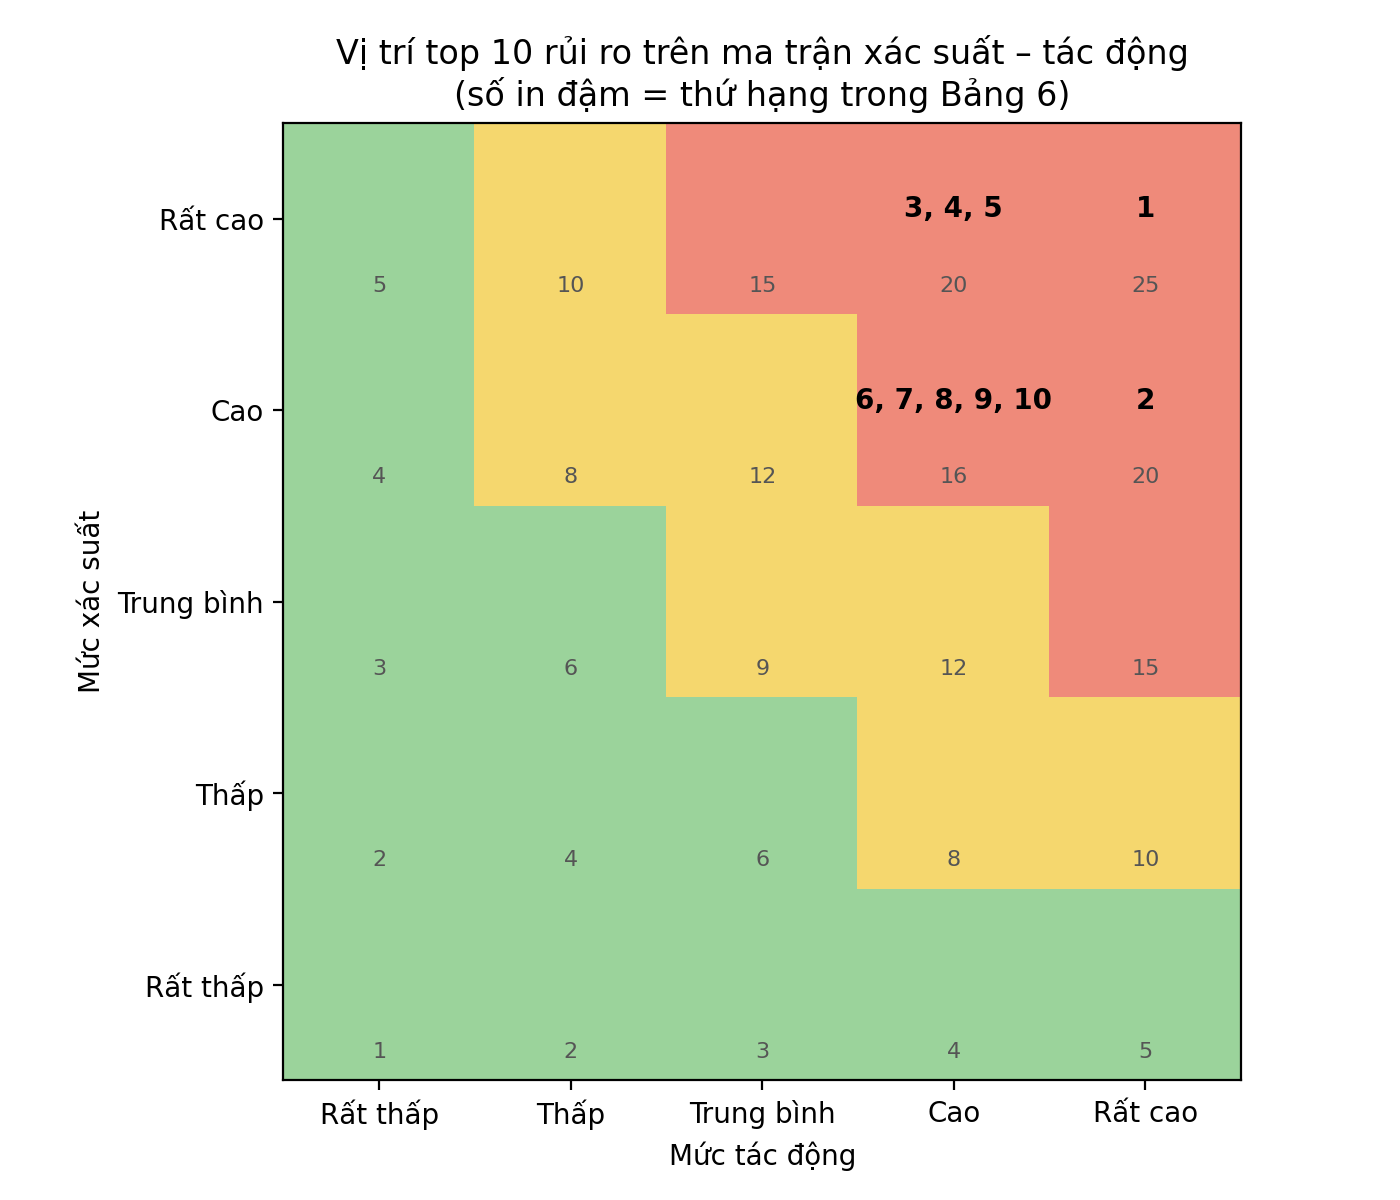
\includegraphics[width=0.72\textwidth]{ma_tran_pim_top10.png}
\caption{Vị trí 10 rủi ro hàng đầu trên ma trận xác suất -- tác động (vẽ lại từ Bảng 6 trong~\cite{kassem2022})}
\label{fig:pim}
\end{figure}

\textbf{So sánh RII và PIM.} Hai công cụ dùng chung đầu vào nhưng trả lời hai câu hỏi khác nhau. RII cho ra một con số liên tục để \emph{xếp hạng}. PIM cho ra một \emph{vùng} để chọn chiến lược ứng phó. Vì PIM chỉ có 5 mức trên mỗi trục, nhiều rủi ro rơi vào cùng một ô: trong Hình~\ref{fig:pim}, năm rủi ro xếp hạng 6 đến 10 cùng nằm ở ô (Cao, Cao) và không phân biệt được với nhau. Ngược lại, RII phân biệt được các yếu tố chỉ chênh nhau vài phần nghìn, nhưng không cho biết nên ứng phó thế nào. Một điểm đáng chú ý là thứ hạng theo hai cách không trùng nhau. Theo RII, ``chính phủ bất ổn'' đứng đầu~\cite{kassem2022}, nhưng yếu tố này không có trong top 10 của ma trận. Chương~\ref{chuong:tai-hien} sẽ kiểm tra lại sự nhất quán giữa hai bảng này.

\section{Mô hình phương trình cấu trúc (SEM)}
\label{sec:sem}

\subsection{Biến tiềm ẩn và biến quan sát}

Nhiều khái niệm trong quản lý dự án không đo trực tiếp được, chẳng hạn ``rủi ro từ phía chủ đầu tư'' hay ``mức độ thành công của dự án''. Những khái niệm như vậy gọi là \textbf{biến tiềm ẩn} (latent variable, construct). Ta chỉ đo được chúng gián tiếp qua các câu hỏi cụ thể gọi là \textbf{biến quan sát} (indicator). Ví dụ, biến tiềm ẩn ``rủi ro chủ đầu tư'' (CL) trong bài báo được đo qua sáu câu CL1--CL6, trong đó CL1 là ``chậm ra quyết định''.

Mô hình phương trình cấu trúc (SEM) là kỹ thuật thống kê đa biến cho phép ước lượng đồng thời hai loại quan hệ~\cite{hair2022primer}:
\begin{itemize}
  \item \textbf{Mô hình đo lường} (mô hình ngoài, outer model): quan hệ giữa mỗi biến tiềm ẩn và các câu hỏi đo nó.
  \item \textbf{Mô hình cấu trúc} (mô hình trong, inner model): quan hệ giữa các biến tiềm ẩn với nhau. Đây chính là các giả thuyết nghiên cứu.
\end{itemize}

Biến tiềm ẩn chỉ đóng vai trò giải thích (không bị biến nào khác tác động) gọi là \textbf{biến ngoại sinh}. Biến tiềm ẩn bị các biến khác tác động gọi là \textbf{biến nội sinh}. Trong bài báo, các nhóm rủi ro là biến ngoại sinh, còn ``ảnh hưởng tới thành công dự án'' là biến nội sinh.

\subsection{Hai cách tiếp cận: CB-SEM và PLS-SEM}

Có hai họ phương pháp ước lượng SEM. CB-SEM (dựa trên hiệp phương sai) tìm bộ tham số sao cho ma trận hiệp phương sai do mô hình tạo ra gần nhất với ma trận hiệp phương sai của dữ liệu, nên phù hợp để \emph{kiểm định một lý thuyết} đã có. PLS-SEM (bình phương tối thiểu riêng phần) tìm bộ tham số sao cho phần phương sai được giải thích của các biến nội sinh là lớn nhất, nên thiên về \emph{giải thích và dự báo}~\cite{hair2022primer,hair2019report}. Bảng~\ref{tab:cb-pls} so sánh hai cách tiếp cận.

\begin{table}[H]
\centering
\caption{So sánh CB-SEM và PLS-SEM (tổng hợp từ~\cite{hair2022primer,hair2019report})}
\label{tab:cb-pls}
\begin{tabularx}{\textwidth}{@{}p{3.6cm}XX@{}}
\toprule
\textbf{Tiêu chí} & \textbf{CB-SEM} & \textbf{PLS-SEM} \\
\midrule
Mục tiêu & Kiểm định, xác nhận lý thuyết & Giải thích phương sai, dự báo, phát triển lý thuyết \\
Giả định phân phối & Cần phân phối chuẩn đa biến & Không cần (phi tham số) \\
Cỡ mẫu & Thường cần lớn (vài trăm trở lên) & Chạy được với mẫu nhỏ hơn \\
Độ phức tạp mô hình & Khó hội tụ khi nhiều biến & Xử lý tốt mô hình nhiều biến, nhiều bậc \\
Độ phù hợp toàn cục & Có ($\chi^2$, CFI, RMSEA\ldots) & Không có chỉ số được thừa nhận rộng rãi \\
Phần mềm phổ biến & AMOS, LISREL, Mplus & SmartPLS, gói seminr (R) \\
\bottomrule
\end{tabularx}
\end{table}

Bài báo chọn PLS-SEM với ba lý do: dữ liệu Likert không có phân phối chuẩn, mô hình phức tạp (51 câu hỏi, 13 nhóm, 2 bậc) và mục tiêu là xác định các yếu tố có ảnh hưởng lớn nhất~\cite{kassem2022}. Lựa chọn này phù hợp với khuyến nghị của Hair và cộng sự~\cite{hair2019report}.

\section{Phương pháp PLS-SEM}
\label{sec:pls-sem}

\subsection{Thuật toán ước lượng}

Thuật toán PLS-SEM ước lượng điểm của mỗi biến tiềm ẩn $Y_j$ như một tổ hợp tuyến tính có trọng số của các câu hỏi đo nó, rồi chạy hồi quy giữa các biến tiềm ẩn. Các trọng số được tìm bằng cách lặp~\cite{hair2022primer,tenenhaus2005}:
\begin{enumerate}
  \item \textbf{Khởi tạo:} gán mọi trọng số ngoài $w_{kj} = 1$.
  \item \textbf{Xấp xỉ ngoài:} tính điểm biến tiềm ẩn từ các câu hỏi rồi chuẩn hóa:
  \begin{equation}
  Y_j = \sum_{k} w_{kj}\, x_{kj}
  \label{eq:xap-xi-ngoai}
  \end{equation}
  \item \textbf{Xấp xỉ trong:} tính một ước lượng khác của mỗi biến tiềm ẩn từ các biến tiềm ẩn kề với nó trong mô hình cấu trúc:
  \begin{equation}
  Z_j = \sum_{i \neq j} e_{ji}\, Y_i
  \label{eq:xap-xi-trong}
  \end{equation}
  trong đó $e_{ji}$ là trọng số trong, tính theo lược đồ đường dẫn (path weighting scheme).
  \item \textbf{Cập nhật trọng số ngoài:} với mô hình đo lường kết quả (reflective, Mode A), trọng số mới là hiệp phương sai giữa câu hỏi và ước lượng trong, $w_{kj} = \operatorname{cov}(x_{kj}, Z_j)$.
  \item \textbf{Lặp lại} bước 2--4 cho tới khi tổng thay đổi của các trọng số nhỏ hơn ngưỡng (SmartPLS mặc định $10^{-7}$).
  \item \textbf{Ước lượng cuối:} loading $\lambda_{kj} = \operatorname{corr}(x_{kj}, Y_j)$. Hệ số đường dẫn $\beta$ là hệ số hồi quy OLS của mỗi biến nội sinh theo các biến tác động lên nó.
\end{enumerate}

\subsection{Bootstrapping và kiểm định giả thuyết}

PLS-SEM không giả định phân phối, nên không có công thức sai số chuẩn như hồi quy thông thường. Sai số chuẩn được ước lượng bằng \textbf{bootstrapping}: rút ngẫu nhiên có hoàn lại $B$ mẫu con (thường $B = 5000$), mỗi mẫu cùng cỡ $n$ với mẫu gốc, chạy lại thuật toán trên từng mẫu để có $B$ giá trị $\hat\beta^{(b)}$. Sai số chuẩn là độ lệch chuẩn của các giá trị đó, và thống kê kiểm định là:
\begin{equation}
t = \frac{\hat\beta}{SE(\hat\beta)}, \qquad SE(\hat\beta) = \sqrt{\frac{1}{B-1}\sum_{b=1}^{B}\left(\hat\beta^{(b)} - \bar{\beta}\right)^2}
\label{eq:bootstrap}
\end{equation}
Với kiểm định hai phía ở mức ý nghĩa 5\%, giả thuyết được ủng hộ khi $|t| > 1{,}96$ (tương ứng $p < 0{,}05$).

\subsection{Đánh giá mô hình đo lường}

Mô hình đo lường kết quả được đánh giá qua độ tin cậy, giá trị hội tụ và giá trị phân biệt~\cite{hair2019report,hair2022primer}:
\begin{itemize}
  \item \textbf{Loading} $\lambda$: mức độ câu hỏi phản ánh biến tiềm ẩn. Ngưỡng $\lambda \geq 0{,}708$, vì khi đó $\lambda^2 \geq 0{,}5$, tức biến tiềm ẩn giải thích ít nhất một nửa phương sai của câu hỏi.
  \item \textbf{Độ tin cậy tổng hợp} (CR):
  \begin{equation}
  CR = \frac{\left(\sum_{k=1}^{K}\lambda_k\right)^2}{\left(\sum_{k=1}^{K}\lambda_k\right)^2 + \sum_{k=1}^{K}\left(1 - \lambda_k^2\right)}
  \label{eq:cr}
  \end{equation}
  Ngưỡng từ 0,70 đến 0,95. Giá trị trên 0,95 là dấu hiệu các câu hỏi trùng lặp nhau.
  \item \textbf{Phương sai trung bình được trích} (AVE), đo giá trị hội tụ:
  \begin{equation}
  AVE = \frac{1}{K}\sum_{k=1}^{K}\lambda_k^2
  \label{eq:ave}
  \end{equation}
  Ngưỡng $AVE \geq 0{,}5$.
  \item \textbf{Giá trị phân biệt}: các biến tiềm ẩn phải thực sự khác nhau. Tiêu chí Fornell--Larcker~\cite{fornell1981} yêu cầu $\sqrt{AVE_j}$ lớn hơn tương quan của biến $j$ với mọi biến tiềm ẩn khác. Henseler và cộng sự~\cite{henseler2015} chỉ ra tiêu chí này thường không phát hiện được vấn đề và đề xuất tỷ số HTMT (trung bình tương quan giữa các câu hỏi khác nhóm chia cho trung bình tương quan giữa các câu hỏi cùng nhóm), với ngưỡng 0,85, hoặc 0,90 với các khái niệm gần nhau.
\end{itemize}

\subsection{Đánh giá mô hình cấu trúc}

\begin{itemize}
  \item \textbf{Hệ số xác định} $R^2$: tỷ lệ phương sai của biến nội sinh được các biến tác động lên nó giải thích. Theo Hair và cộng sự~\cite{hair2019report}, các mức 0,75 / 0,50 / 0,25 tương ứng mạnh / trung bình / yếu. Chin~\cite{chin1998} dùng các mức 0,67 / 0,33 / 0,19.
  \item \textbf{Quy mô tác động} $f^2$: mức giảm $R^2$ khi bỏ một biến ngoại sinh khỏi mô hình,
  \begin{equation}
  f^2 = \frac{R^2_{co} - R^2_{bo}}{1 - R^2_{co}}
  \label{eq:f2}
  \end{equation}
  với các mức 0,02 / 0,15 / 0,35 tương ứng nhỏ / trung bình / lớn~\cite{cohen1988}.
  \item \textbf{Mức liên quan dự báo} $Q^2$, tính bằng thủ tục blindfolding: lần lượt che một phần dữ liệu, dự báo lại phần bị che rồi so sánh,
  \begin{equation}
  Q^2 = 1 - \frac{SSE}{SSO}
  \label{eq:q2}
  \end{equation}
  trong đó $SSE$ là tổng bình phương sai số dự báo và $SSO$ là tổng bình phương các giá trị quan sát, bằng $n \times K$ với $K$ là số câu hỏi của biến. Mô hình có khả năng dự báo khi $Q^2 > 0$.
  \item \textbf{Chỉ số phù hợp} GoF do Tenenhaus và cộng sự~\cite{tenenhaus2005} đề xuất:
  \begin{equation}
  GoF = \sqrt{\overline{AVE} \times \overline{R^2}}
  \label{eq:gof}
  \end{equation}
  Bài báo dùng ngưỡng 0,36 để kết luận mô hình phù hợp. Tuy nhiên Henseler và Sarstedt~\cite{henseler2013} đã chỉ ra GoF không phân biệt được mô hình đúng với mô hình sai, và Hair và cộng sự~\cite{hair2019report} khuyến nghị không dùng chỉ số này.
\end{itemize}

\section{Mô hình nghiên cứu của bài báo}
\label{sec:mo-hinh}

Mô hình của bài báo (Hình~\ref{fig:mo-hinh}) là một mô hình \textbf{hai bậc}. Ở bậc 1, 51 câu hỏi đo 13 nhóm rủi ro. Ở bậc 2, 13 nhóm này được gom thành hai khái niệm tổng quát hơn: \emph{rủi ro nội bộ} gồm 7 nhóm (chủ đầu tư, nhà thầu, tư vấn, khả thi và thiết kế, đấu thầu và hợp đồng, nguồn lực và vật tư, quản lý dự án) và \emph{rủi ro bên ngoài} gồm 6 nhóm (kinh tế, chính trị, người dân địa phương, môi trường và an toàn, an ninh, bất khả kháng). Hai khái niệm bậc 2 cùng tác động lên biến nội sinh \emph{ảnh hưởng của rủi ro tới thành công dự án}, đo bằng năm hậu quả EF1--EF5.

\begin{figure}[H]
\centering
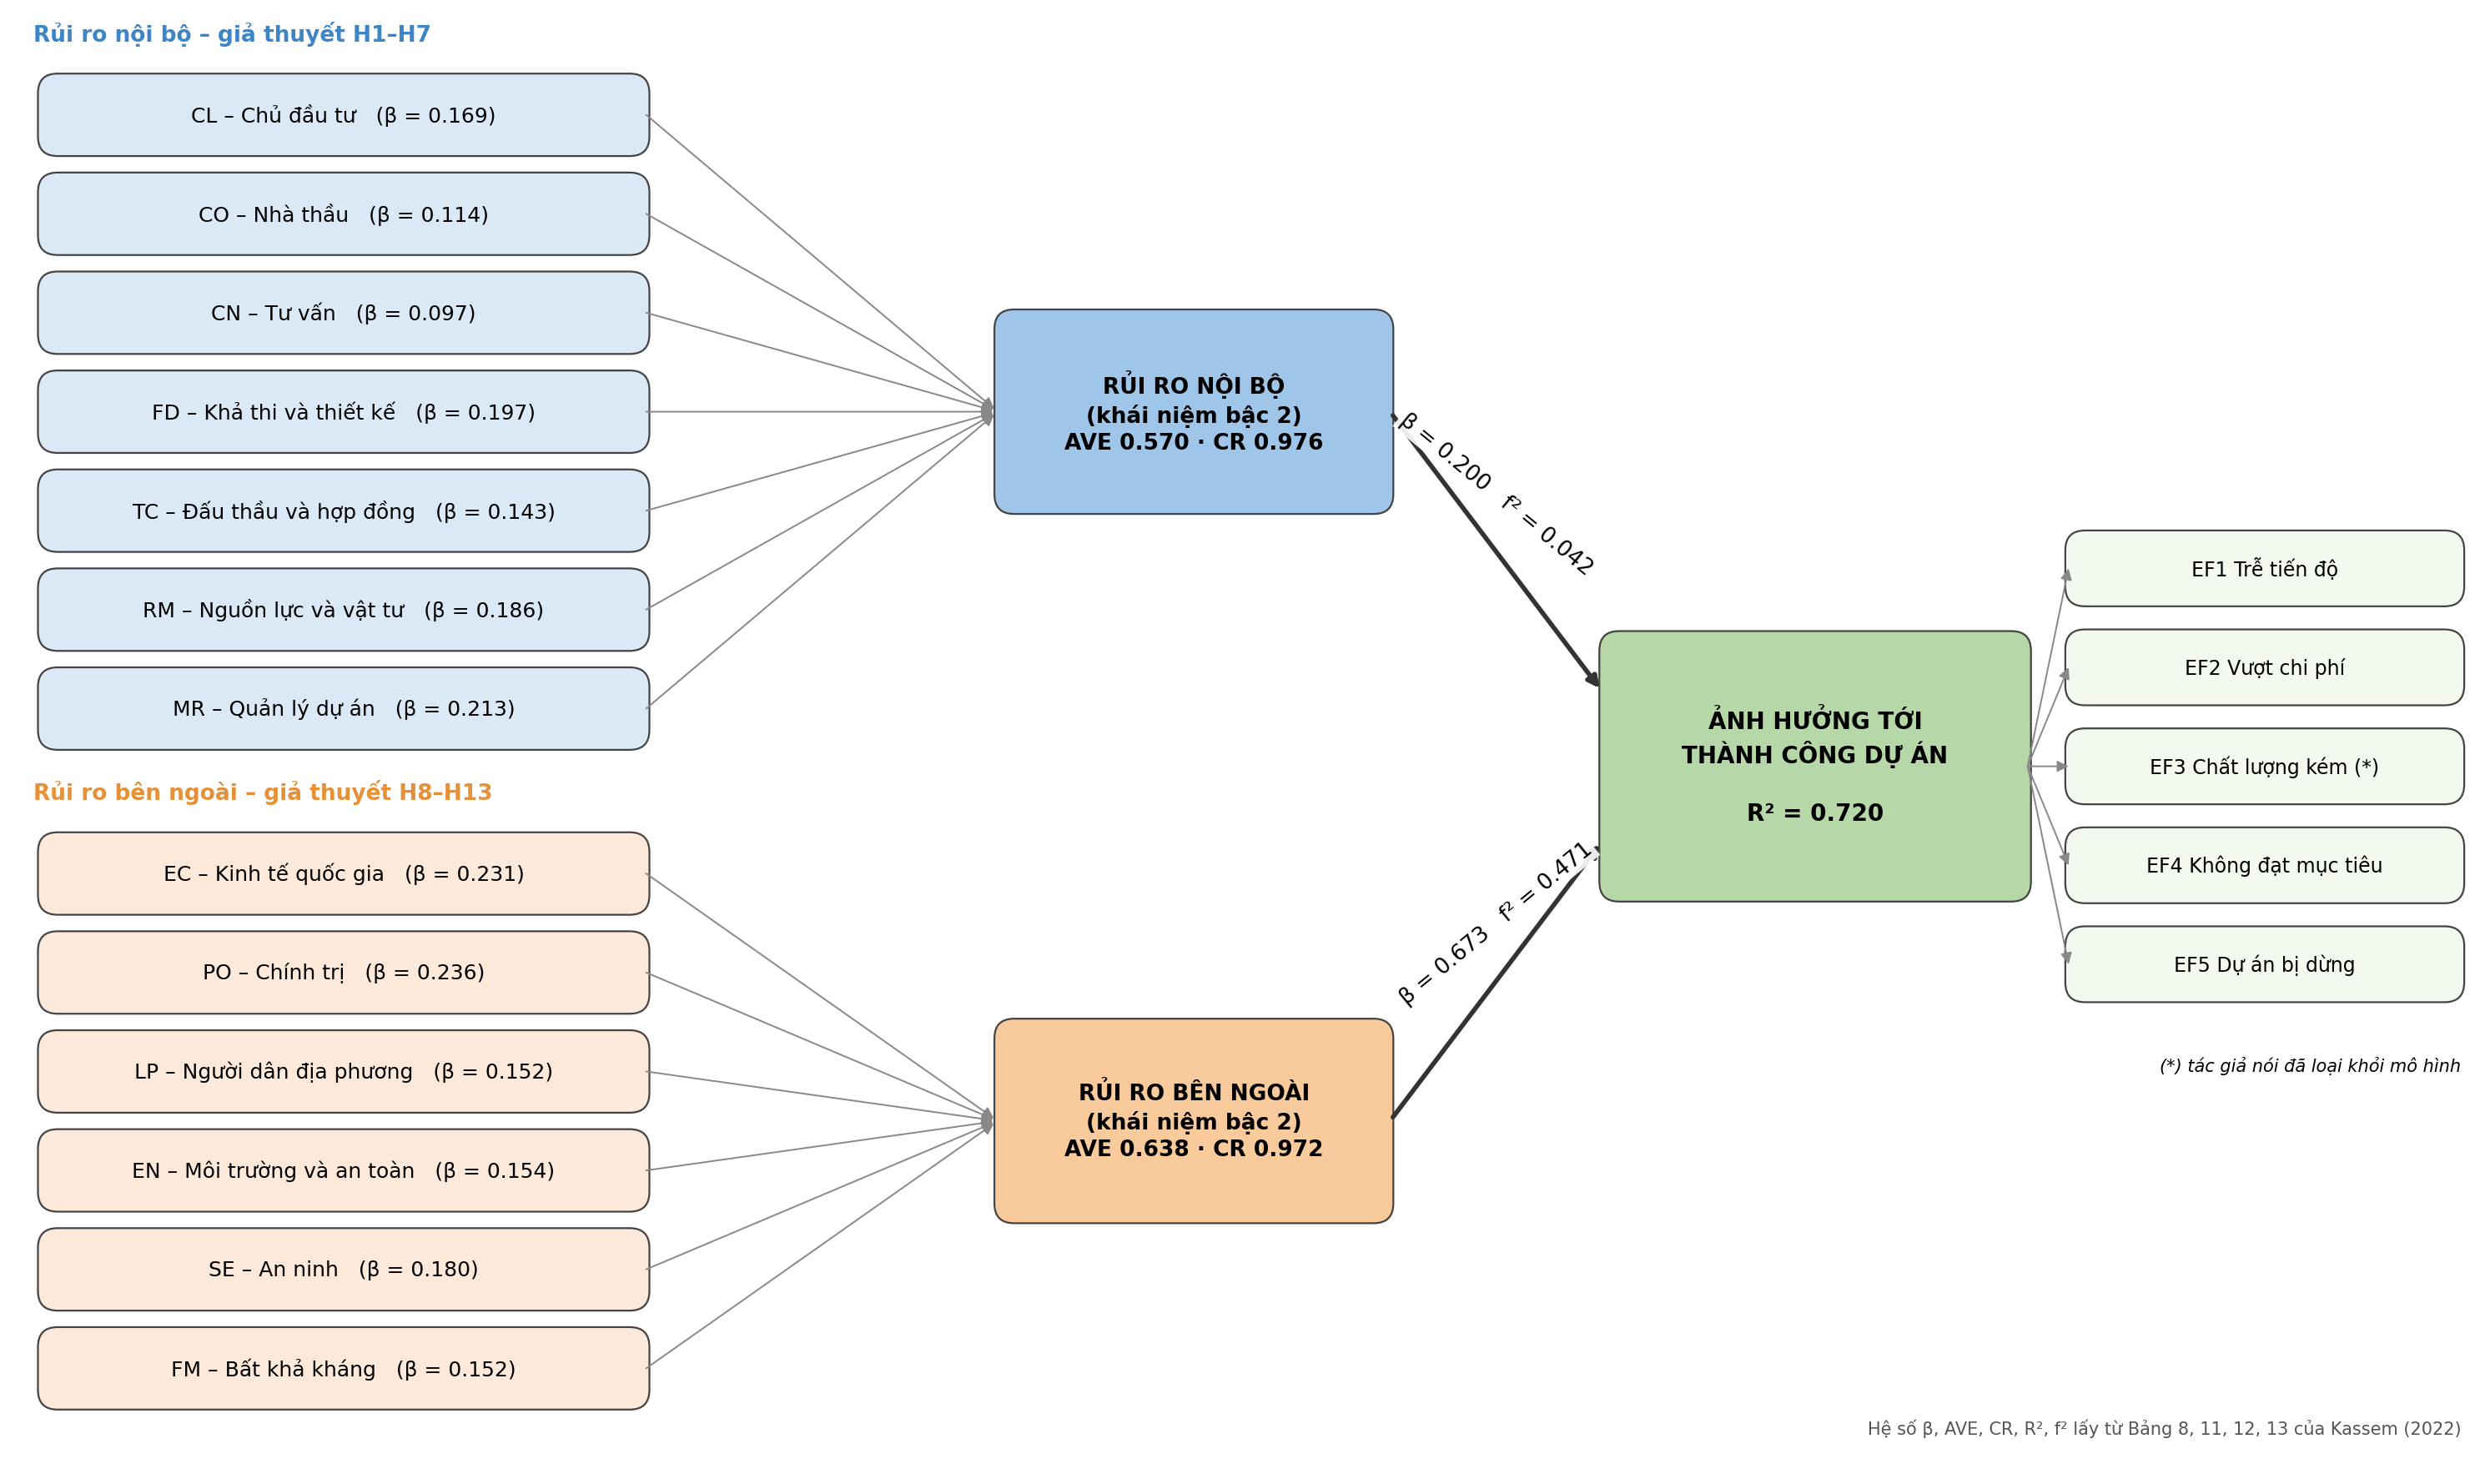
\includegraphics[width=\textwidth]{mo_hinh_nghien_cuu.png}
\caption{Mô hình nghiên cứu hai bậc và các hệ số do bài báo công bố (vẽ lại từ~\cite{kassem2022})}
\label{fig:mo-hinh}
\end{figure}

Tác giả phát biểu 13 giả thuyết H1--H13 có chung dạng ``nhóm rủi ro X ảnh hưởng tới thành công của dự án xây dựng'', mỗi giả thuyết ứng với một nhóm. Phần thảo luận còn nhắc tới H14 và H15 mà không định nghĩa. Căn cứ vào ngữ cảnh, đó là hai đường dẫn từ rủi ro nội bộ và rủi ro bên ngoài tới thành công dự án.

Khi đọc mô hình cần lưu ý hai điểm:
\begin{enumerate}
  \item Biến nội sinh được đo bằng các \emph{hậu quả xấu}: điểm càng cao thì dự án càng chịu nhiều tác động tiêu cực. Vì vậy hệ số $\beta$ dương nghĩa là rủi ro càng lớn thì dự án càng \emph{kém} thành công.
  \item Trong mô hình hai bậc, các nhóm bậc 1 không nối trực tiếp tới biến nội sinh mà đi qua khái niệm bậc 2. Có nhiều cách ước lượng loại mô hình này, như lặp chỉ báo (repeated indicators) hay hai giai đoạn (two-stage), và mỗi cách cho kết quả khác nhau~\cite{sarstedt2019hoc}. Bài báo không nói đã dùng cách nào, nên không rõ 13 hệ số $\beta$ của từng nhóm được tính ra sao. Chương~\ref{chuong:tai-hien} sẽ phân tích kỹ hơn điểm này.
\end{enumerate}

\section{Ứng dụng, ưu điểm, hạn chế và xu hướng}
\label{sec:danh-gia-pp}

\subsection{Ứng dụng}

PLS-SEM được dùng nhiều trong marketing, hệ thống thông tin (ví dụ các mô hình chấp nhận công nghệ), quản trị chiến lược, và ngày càng phổ biến trong quản lý xây dựng~\cite{hair2022primer}. Trong quản lý dự án, phương pháp này thường được dùng để mô hình hóa nguyên nhân chậm tiến độ, vượt chi phí và rủi ro~\cite{kassem2022}. Ngay trong lĩnh vực hệ thống thông tin, đã có nghiên cứu dùng SEM để phân tích ảnh hưởng của mức độ không chắc chắn và quản lý rủi ro lên kết quả của dự án phát triển hệ thống thông tin (tài liệu [15] trong~\cite{kassem2022}).

\subsection{Ưu điểm}

\begin{itemize}
  \item Không đòi hỏi phân phối chuẩn, phù hợp với dữ liệu khảo sát thang Likert.
  \item Chạy được mô hình nhiều biến, nhiều bậc mà CB-SEM khó hội tụ.
  \item Cho ra điểm số cụ thể của từng biến tiềm ẩn, dùng được cho các phân tích tiếp theo.
  \item Kết hợp được với RII và PIM: RII và PIM trả lời câu hỏi ``rủi ro nào quan trọng'', còn PLS-SEM trả lời ``nhóm rủi ro nào ảnh hưởng tới kết quả dự án và mạnh đến đâu''.
\end{itemize}

\subsection{Hạn chế}

\begin{itemize}
  \item Với mô hình đo lường kết quả, PLS-SEM có xu hướng ước lượng loading cao hơn và hệ số đường dẫn thấp hơn giá trị thật. Phiên bản PLS nhất quán (PLSc) được đề xuất để khắc phục~\cite{dijkstra2015}.
  \item Không có chỉ số phù hợp toàn cục được thừa nhận. Việc dùng GoF như bài báo không còn được khuyến nghị~\cite{henseler2013}.
  \item Kết quả phụ thuộc vào chất lượng dữ liệu khảo sát. Nếu người trả lời chấm theo một cảm nhận chung (ví dụ ``mọi thứ ở Yemen đều rủi ro''), các nhóm sẽ tương quan cao với nhau và giá trị phân biệt bị ảnh hưởng.
  \item Mô hình chỉ cho thấy mối liên hệ thống kê. Dữ liệu cắt ngang từ một lần khảo sát không đủ để khẳng định quan hệ nhân quả theo nghĩa chặt chẽ.
\end{itemize}

\subsection{Xu hướng}

\begin{itemize}
  \item \textbf{Đánh giá khả năng dự báo ngoài mẫu} bằng PLSpredict, thay cho $Q^2$ tính trong mẫu~\cite{shmueli2019}.
  \item \textbf{Dùng HTMT} thay cho Fornell--Larcker làm tiêu chí giá trị phân biệt chính~\cite{henseler2015}.
  \item \textbf{Chuẩn hóa cách xây dựng mô hình bậc cao}~\cite{sarstedt2019hoc}.
  \item \textbf{Công cụ mã nguồn mở} như gói seminr trên R giúp người khác tái hiện được kết quả~\cite{hair2021workbook}. Điều này đặc biệt quan trọng khi dữ liệu gốc không được công bố, như trường hợp của bài báo này.
\end{itemize}

\chapter{Tái hiện thực nghiệm}
\label{chuong:tai-hien}

Chương này tái hiện lại phần phân tích dữ liệu của bài báo. Toàn bộ mã nguồn, số liệu và kết quả được lưu trên GitHub (Phụ lục~A), và mọi con số trong chương đều được sinh ra từ các script ở thư mục \texttt{src/}.

\section{Quy trình tái hiện}
\label{sec:quy-trinh}

Khó khăn lớn nhất là bài báo \textbf{không công bố dữ liệu gốc}. Mục ``Data Availability Statement'' chỉ ghi rằng dữ liệu được cung cấp khi có yêu cầu hợp lý~\cite{kassem2022}. Vì vậy báo cáo tái hiện theo hai hướng bổ sung cho nhau (Hình~\ref{fig:quy-trinh}):
\begin{itemize}
  \item \textbf{Hướng 1 -- Kiểm tra số liệu đã công bố.} Gõ lại 10 bảng số liệu của bài báo, tính lại mọi chỉ số tính lại được từ chính các bảng đó, rồi đối chiếu với số đã in. Hướng này trả lời câu hỏi: \emph{các con số trong bài có nhất quán với nhau không?}
  \item \textbf{Hướng 2 -- Phân tích trên dữ liệu mô phỏng.} Sinh một bộ 314 phiếu khảo sát giả lập, có tương quan, loading và hệ số đúng như bài báo công bố, rồi chạy lại toàn bộ quy trình phân tích. Hướng này trả lời câu hỏi: \emph{nếu dữ liệu thật có cấu trúc như bài báo mô tả, thì quy trình chuẩn sẽ cho ra kết quả như thế nào?}
\end{itemize}

\begin{figure}[H]
\centering
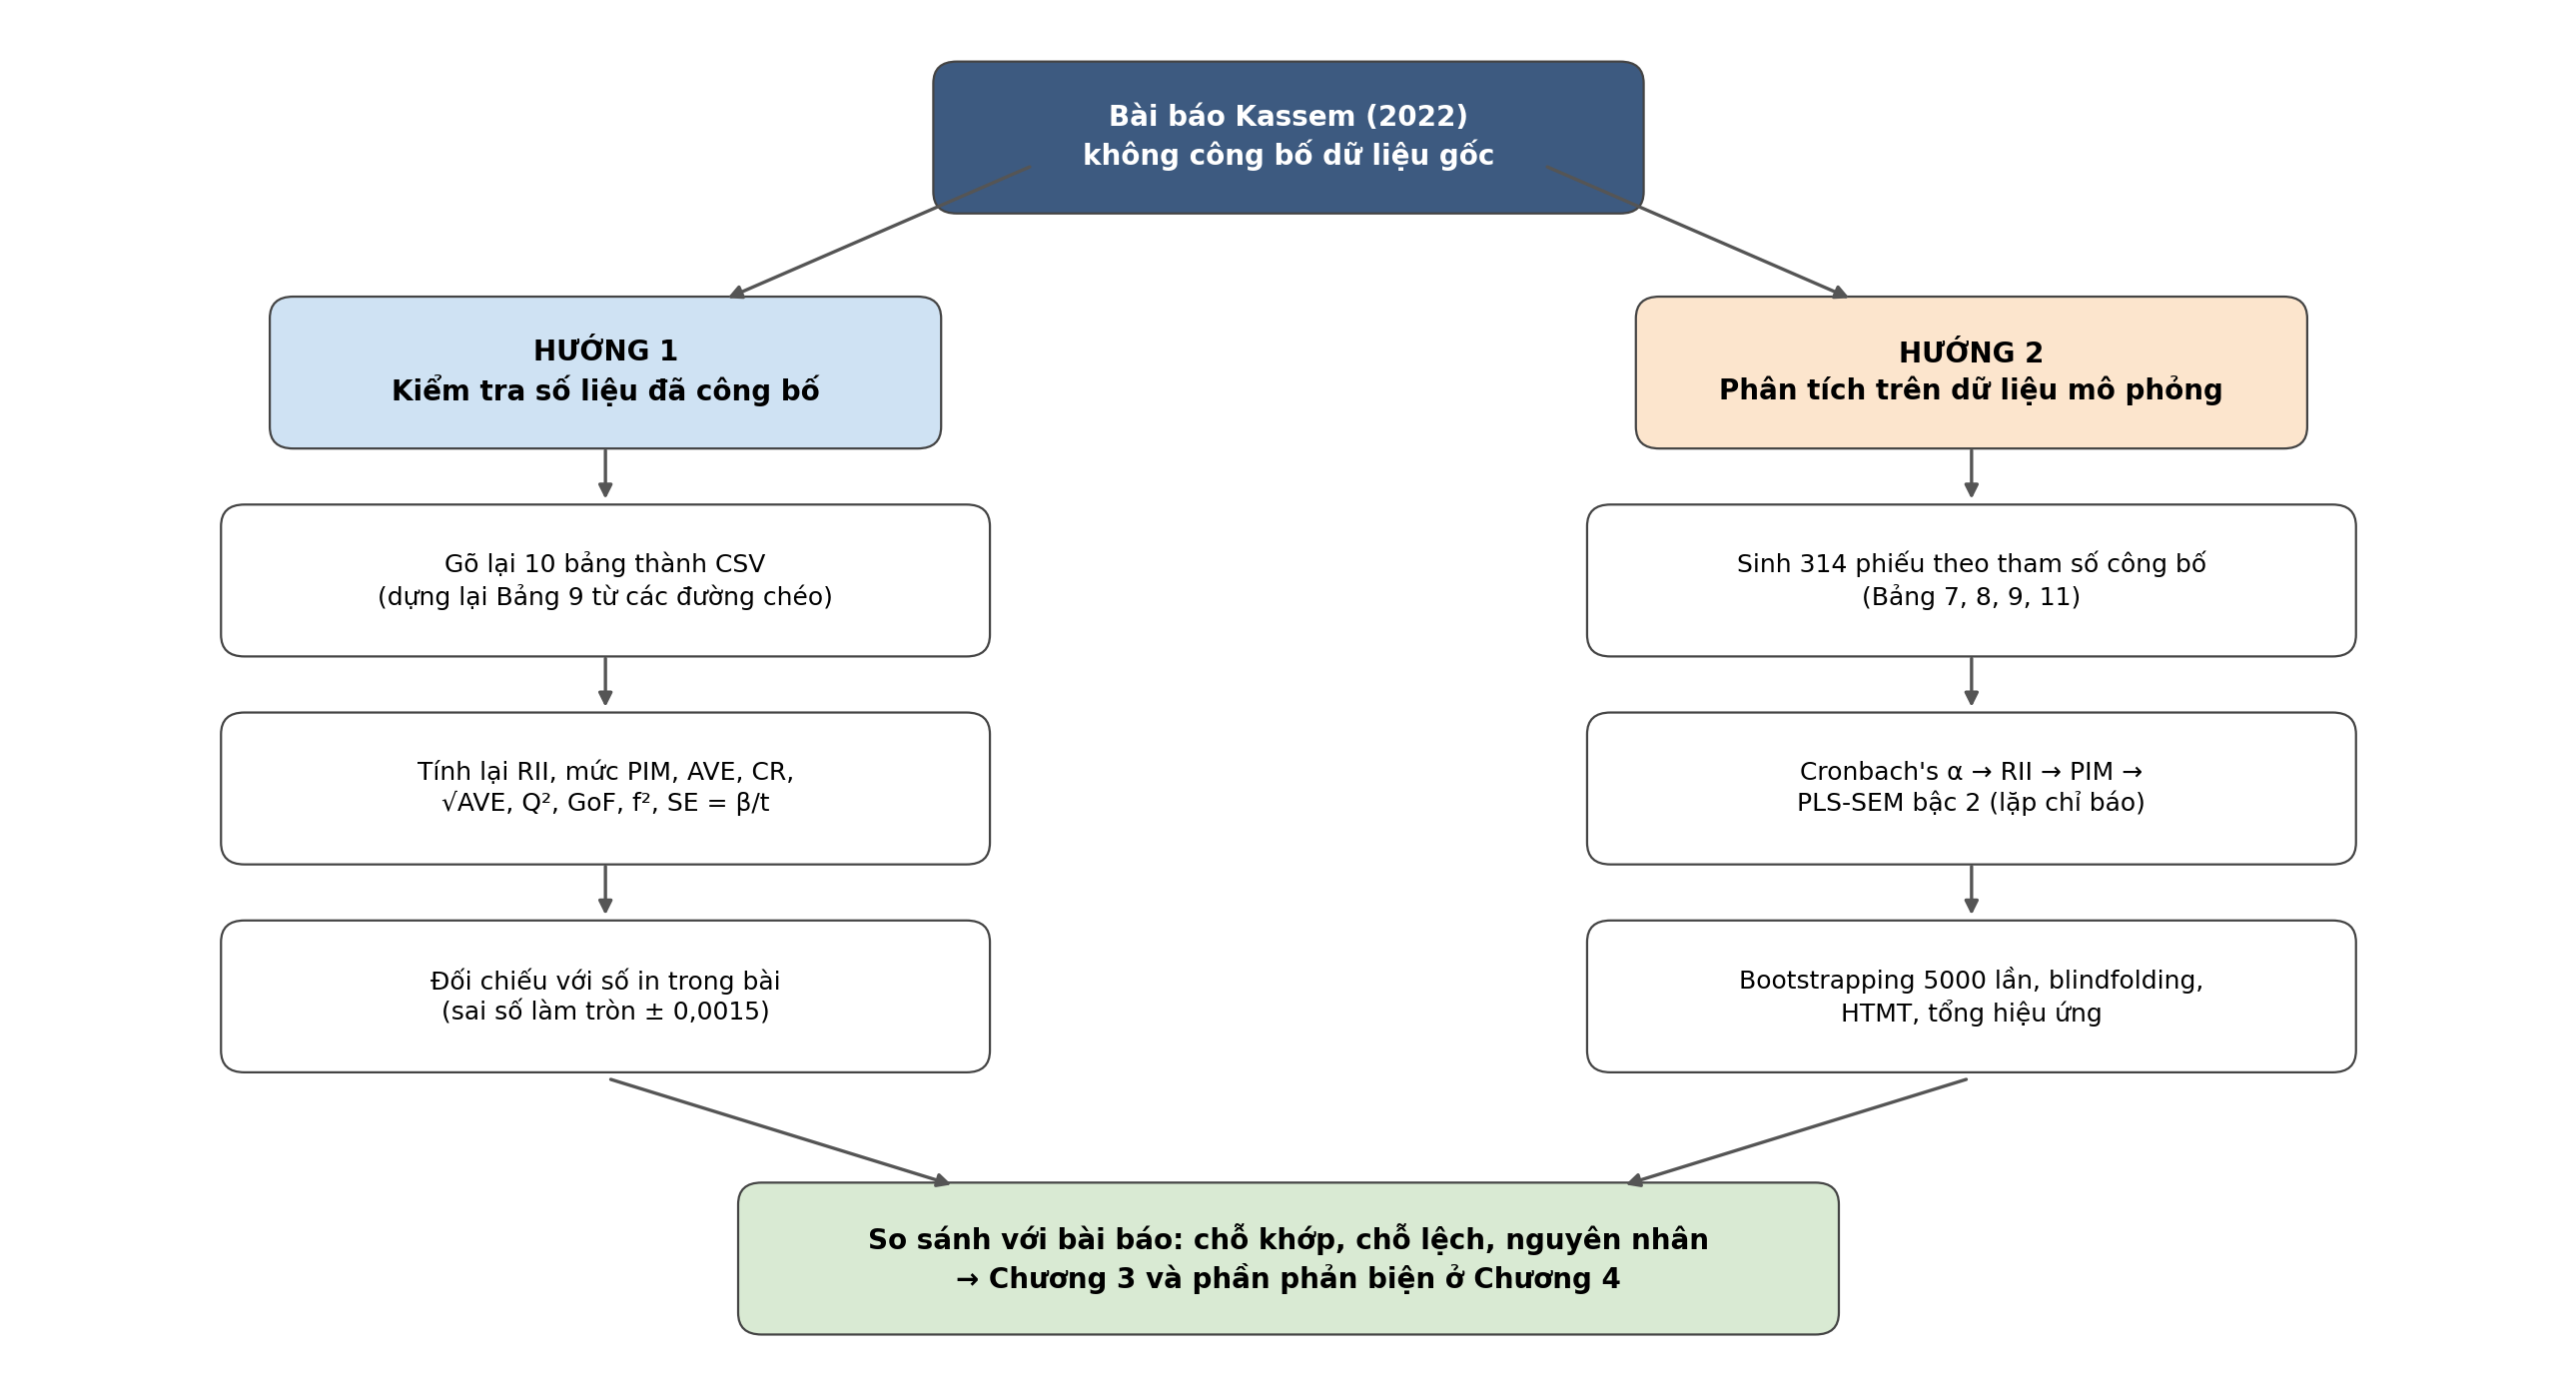
\includegraphics[width=\textwidth]{quy_trinh_tai_hien.png}
\caption{Quy trình tái hiện thực nghiệm theo hai hướng}
\label{fig:quy-trinh}
\end{figure}

\textbf{Công cụ.} Bài báo dùng SPSS v25 và SmartPLS 3, đều là phần mềm thương mại. Báo cáo dùng Python 3 với các thư viện mã nguồn mở numpy, pandas và matplotlib. Thuật toán PLS-SEM, bootstrapping, blindfolding và HTMT được tự cài đặt theo đúng các bước ở mục~\ref{sec:pls-sem}. Để kiểm tra phần cài đặt, mô hình được chạy thử trên một bộ dữ liệu biết trước đáp án: hai biến tiềm ẩn, mỗi biến 4 câu hỏi có loading thật 0,85, hệ số đường dẫn thật 0,6, cỡ mẫu 2000. Kết quả cho loading 0,88--0,89 và hệ số đường dẫn 0,544. Như vậy loading bị ước lượng cao hơn và hệ số đường dẫn thấp hơn giá trị thật, đúng với tính chất đã biết của PLS-SEM~\cite{dijkstra2015}.

\section{Kiểm tra số liệu đã công bố}
\label{sec:kiem-tra}

\subsection{Nhập số liệu}

Mười bảng của bài báo (Bảng 5 tới Bảng 14) được gõ lại thành file CSV. Nhiều bảng trong bản PDF bị lệch cột hoặc lệch hàng, nên phải căn chỉnh lại:
\begin{itemize}
  \item Bảng 5: cột số câu hỏi và cột $\alpha$ bị đẩy xuống một dòng. Căn lại sao cho tổng số câu bằng 51.
  \item Bảng 7: các cột RII tác động và RII xác suất không thẳng hàng với tên rủi ro. Căn lại theo thứ tự dòng, rồi kiểm tra bằng phép nhân ở mục~\ref{sec:kt-rii}.
  \item Bảng 9: ma trận Fornell--Larcker bị in theo từng \emph{đường chéo}. Dòng đầu tiên là đường chéo chính ($\sqrt{AVE}$), dòng thứ hai là đường chéo kế tiếp, v.v. Ma trận được dựng lại thành dạng tam giác dưới $13 \times 13$. Kết quả hợp lý: đường chéo trùng với $\sqrt{AVE}$ tính từ Bảng 8, và ma trận đầy đủ là xác định dương (trị riêng nhỏ nhất bằng 0,092).
  \item Bảng 11: tên các nhóm và các giá trị bị lệch hàng. Ghép lại theo thứ tự chữ cái tiếng Anh của Hình 8 trong bài báo.
\end{itemize}

Bảng~\ref{tab:tong-hop-kiem-tra} tóm tắt kết quả của chín phép kiểm tra. Các mục tiếp theo trình bày chi tiết.

\begin{table}[H]
\centering
\caption{Tổng hợp kết quả kiểm tra số liệu đã công bố}
\label{tab:tong-hop-kiem-tra}
\begin{tabularx}{\textwidth}{@{}clXc@{}}
\toprule
\textbf{TT} & \textbf{Phép kiểm tra} & \textbf{Kết quả} & \textbf{Đánh giá} \\
\midrule
1 & $RII_{tong} = RII_I \times RII_P$ (Bảng 7) & 10/10 dòng khớp, thứ hạng giữ nguyên & Khớp \\
2 & Mức PIM (Bảng 6) so với RII (Bảng 7) & 3/6 rủi ro khớp & Lệch \\
3 & AVE, CR của 13 nhóm từ loading (Bảng 8) & 13/13 khớp & Khớp \\
4 & AVE của biến kết quả EF & 0,494 so với 0,549 & Lệch \\
5 & Fornell--Larcker (Bảng 9) & Nhóm RM không đạt & Lệch \\
6 & Sai số chuẩn suy ra $\beta / t$ (Bảng 11) & Nhỏ bất thường (0,003--0,006) & Nghi vấn \\
7 & $Q^2 = 1 - SSE/SSO$ (Bảng 14) & 3/3 khớp & Khớp \\
8 & GoF (mục 4.3.6e) & Khớp 0,638 nhưng không rõ AVE 0,566 & Nghi vấn \\
9 & $R^2$, $f^2$ so với tương quan ở Bảng 9 & Gần khớp & Khớp \\
\bottomrule
\end{tabularx}
\end{table}

\subsection{RII và ma trận xác suất -- tác động}
\label{sec:kt-rii}

Nhân RII tác động với RII xác suất của 10 rủi ro hàng đầu (công thức~\eqref{eq:rii-tong}) cho ra đúng RII tổng mà bài báo công bố ở cả 10 dòng, với sai lệch không quá 0,0007 do làm tròn. Thứ hạng tính lại cũng giống hệt (Hình~\ref{fig:rii-top10}). Kết quả này xác nhận cách hiểu ở mục~\ref{sec:rii}: $W$ trong công thức~\eqref{eq:rii} là tổng điểm chứ không phải điểm trung bình như bài báo viết.

\begin{figure}[H]
\centering
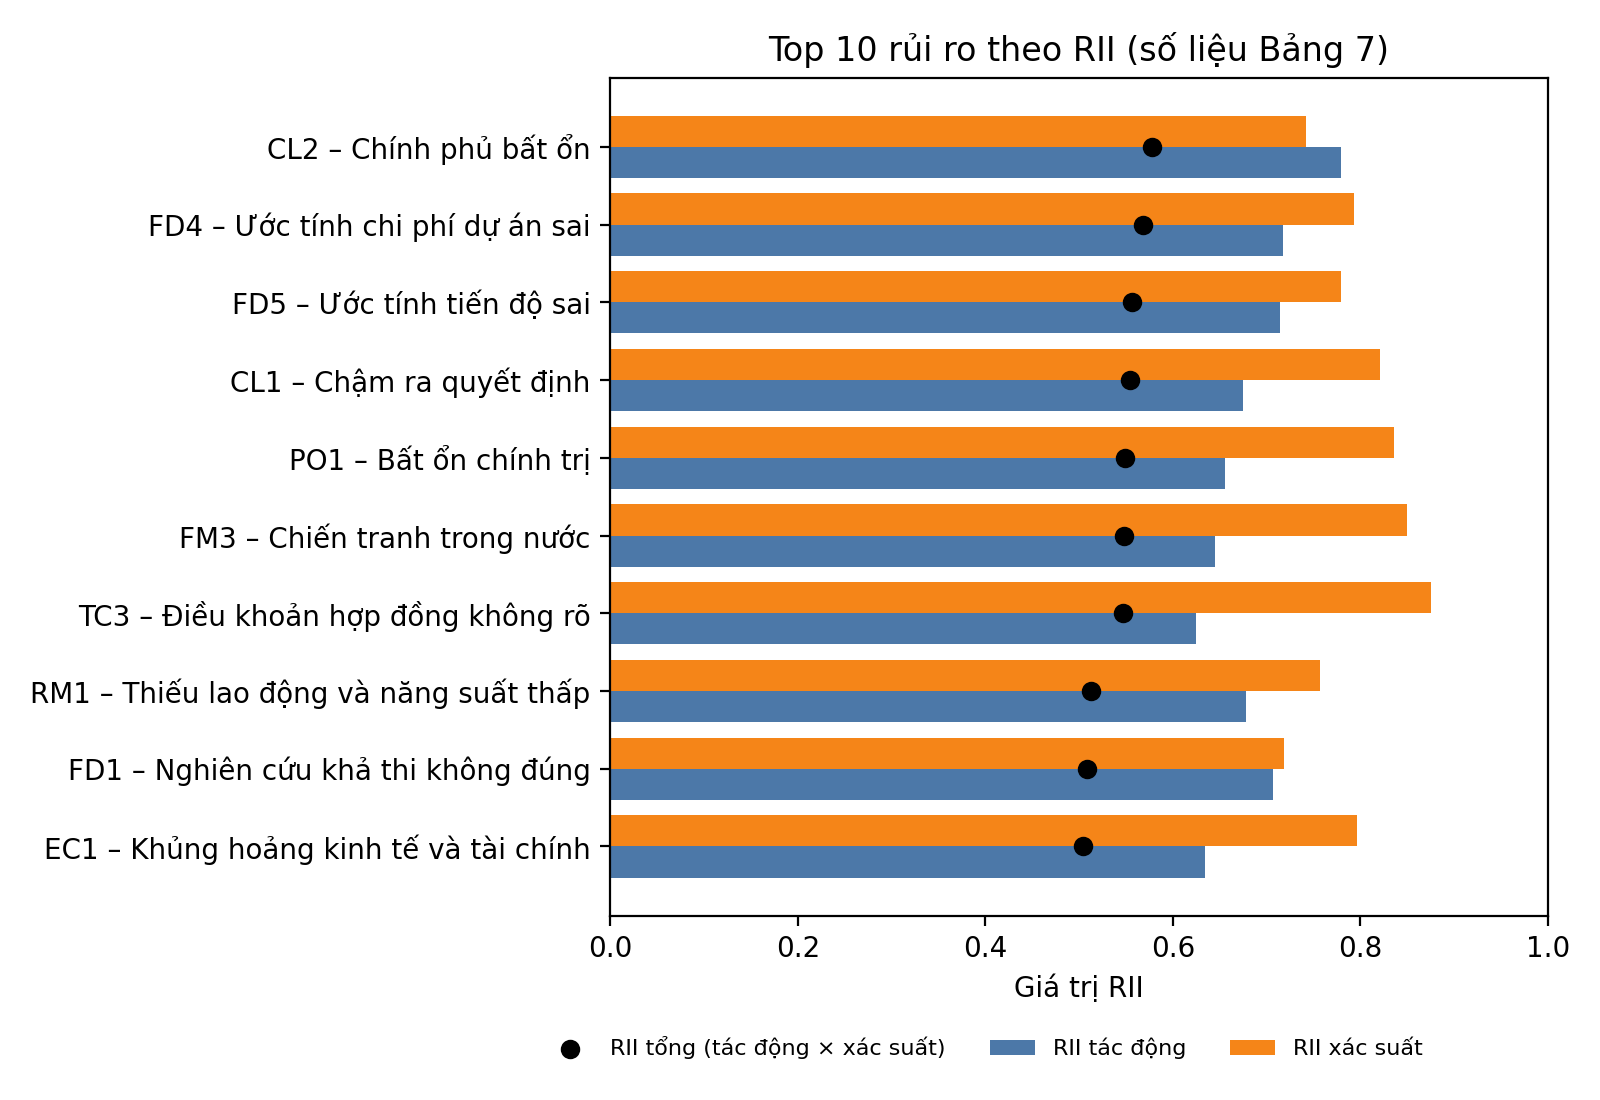
\includegraphics[width=0.85\textwidth]{rii_top10.png}
\caption{RII tác động, RII xác suất và RII tổng của 10 rủi ro hàng đầu (số liệu Bảng 7 trong~\cite{kassem2022})}
\label{fig:rii-top10}
\end{figure}

Ngược lại, ma trận xác suất -- tác động (Bảng 6) \emph{không nhất quán} với RII (Bảng 7). Bài báo không nói cách quy đổi từ điểm sang 5 mức. Nếu dùng cách chia đều thông dụng (mỗi mức rộng 0,2 trên thang RII), thì chỉ 3 trong 6 rủi ro có mặt ở cả hai bảng có mức trùng nhau (Bảng~\ref{tab:pim-rii}). Ví dụ, ``ước tính chi phí sai'' (FD4) có RII tác động 0,717 và RII xác suất 0,793, tức cả hai đều ở mức Cao, nhưng Bảng 6 xếp nó vào ô Rất cao -- Rất cao. Ngoài ra, ``chính phủ bất ổn'' (CL2) đứng đầu theo RII nhưng không có mặt trong top 10 của ma trận.

\begin{table}[H]
\centering
\caption{Mức tác động và xác suất trong Bảng 6 so với mức quy đổi từ RII ở Bảng 7}
\label{tab:pim-rii}
\begin{tabular}{@{}cccccccc@{}}
\toprule
\multirow{2}{*}{\textbf{Mã}} & \multicolumn{2}{c}{\textbf{Bảng 6}} & \multicolumn{2}{c}{\textbf{RII (Bảng 7)}} & \multicolumn{2}{c}{\textbf{Quy đổi}} & \multirow{2}{*}{\textbf{Khớp}} \\
\cmidrule(lr){2-3}\cmidrule(lr){4-5}\cmidrule(lr){6-7}
 & Tác động & Xác suất & Tác động & Xác suất & Tác động & Xác suất & \\
\midrule
FD4 & VH & VH & 0,717 & 0,793 & H & H & Không \\
FD5 & VH & H  & 0,714 & 0,779 & H & H & Không \\
PO1 & H  & VH & 0,656 & 0,836 & H & VH & Có \\
FD1 & H  & VH & 0,707 & 0,718 & H & H & Không \\
CL1 & H  & VH & 0,675 & 0,821 & H & VH & Có \\
RM1 & H  & H  & 0,678 & 0,757 & H & H & Có \\
\bottomrule
\end{tabular}
\end{table}

\subsection{Mô hình đo lường}

\textbf{AVE và CR.} Tính lại AVE và CR của 13 nhóm rủi ro từ 51 loading trong Bảng 8 theo các công thức~\eqref{eq:ave} và~\eqref{eq:cr} cho kết quả khớp hoàn toàn với số bài báo công bố (13/13 nhóm). Riêng biến kết quả EF, năm loading in trong bảng (0,595; 0,761; 0,741; 0,800; 0,591) cho $AVE = 0{,}494$, \emph{dưới} ngưỡng 0,5, trong khi bài báo in 0,549. Tác giả cho biết đã loại câu EF3 (chất lượng kém). Tuy nhiên, thử bỏ lần lượt từng câu thì AVE cao nhất chỉ đạt 0,531 (khi bỏ EF3), không có trường hợp nào bằng 0,549.

\textbf{Fornell--Larcker.} Với ma trận Bảng 9 đã dựng lại, so sánh $\sqrt{AVE}$ của mỗi nhóm với tương quan lớn nhất của nhóm đó cho thấy:
\begin{itemize}
  \item Nhóm \textbf{RM} (nguồn lực và vật tư) \textbf{không đạt}: tương quan với nhóm MR (quản lý dự án) là 0,845, lớn hơn $\sqrt{AVE_{RM}} = 0{,}833$. Bài báo lại kết luận mọi nhóm đều đạt.
  \item Bốn nhóm đạt sát ngưỡng, chênh lệch dưới 0,03: CL (+0,002 so với CO), EC (+0,012 so với PO), PO (+0,019 so với EC), TC (+0,020 so với FD).
  \item Trung bình tương quan giữa các nhóm là 0,712; có 8 trong 78 cặp vượt 0,80.
\end{itemize}
Đây là phát hiện quan trọng nhất của hướng 1, vì chỉ dùng chính số liệu của bài báo. Các nhóm rủi ro chồng lấn nhau nhiều, nhất là cặp RM -- MR và cụm kinh tế -- chính trị -- an ninh. Bài báo không báo cáo HTMT, nên không kiểm tra được mức độ nghiêm trọng của vấn đề này (xem mục~\ref{sec:mo-phong}).

\subsection{Mô hình cấu trúc}

\textbf{Sai số chuẩn của hệ số đường dẫn.} Bảng 11 cho cả $\beta$ và $t$, nên suy ra được sai số chuẩn bootstrap $SE = \beta / t$. Hai đường dẫn bậc 2 (nội bộ và bên ngoài tới EF) có $SE \approx 0{,}064$, là mức hợp lý với cỡ mẫu 314. Nhưng 13 nhóm bậc 1 có $SE$ chỉ từ 0,003 đến 0,006, nhỏ hơn 10 đến 20 lần, dẫn tới các giá trị $t$ rất lớn (26 đến 44). Bài báo không giải thích 13 hệ số này được ước lượng ra sao.

\textbf{$Q^2$.} Tính lại $Q^2 = 1 - SSE/SSO$ từ Bảng 14 khớp cả ba dòng. Bảng 14 không ghi rõ dòng nào ứng với biến nào, nhưng vì $SSO = n \times K$ (mục~\ref{sec:pls-sem}), lấy $SSO$ chia cho 314 sẽ ra số câu hỏi $K$ của biến: 1256/314 = 4 câu (biến EF sau khi bỏ EF3), 6280/314 = 20 câu (rủi ro bên ngoài), 9734/314 = 31 câu (rủi ro nội bộ). Như vậy $Q^2$ của rủi ro nội bộ là 0,527 và bên ngoài là 0,590. Mục 5.3 của bài báo ghi đúng, còn phần Kết luận ghi ngược.

\textbf{GoF.} $\sqrt{0{,}720 \times 0{,}566} = 0{,}638$, khớp với số bài báo công bố. Tuy nhiên, bài báo không nói 0,566 là trung bình AVE của những biến nào. Thử sáu cách lấy trung bình (13 nhóm bậc 1; 13 nhóm và EF; hai nhóm bậc 2; hai nhóm bậc 2 và EF; v.v.) đều không ra 0,566. Theo cách phổ biến nhất (trung bình AVE của các nhóm bậc 1), GoF sẽ xấp xỉ 0,735.

\textbf{Tính nhất quán giữa $R^2$, $\beta$ và $f^2$.} Với hai biến giải thích chuẩn hóa có tương quan $r$, hệ số xác định và hệ số xác định khi bỏ một biến lần lượt là:
\begin{equation}
R^2 = \beta_1^2 + \beta_2^2 + 2\beta_1\beta_2 r, \qquad R^2_{bo\,1} = (\beta_2 + \beta_1 r)^2
\label{eq:r2-hai-bien}
\end{equation}
Lấy $r$ là tương quan giữa trung bình 7 nhóm nội bộ và trung bình 6 nhóm bên ngoài, tính từ ma trận Bảng 9, ta được $r \approx 0{,}831$. Thay $\beta_1 = 0{,}200$ và $\beta_2 = 0{,}673$ vào~\eqref{eq:r2-hai-bien} và~\eqref{eq:f2} được $R^2 = 0{,}717$ (bài báo: 0,720), $f^2_{noi\,bo} = 0{,}044$ (bài báo: 0,042) và $f^2_{ben\,ngoai} = 0{,}494$ (bài báo: 0,471). Vì $r$ chỉ là xấp xỉ (bài báo dùng trọng số PLS chứ không lấy trung bình đều), có thể kết luận phần mô hình cấu trúc bậc 2 \emph{gần như nhất quán} với số liệu tương quan của chính bài báo.

\subsection{Nhận xét}

Phần tính toán cơ bản của bài báo là đúng: RII, AVE và CR của các nhóm, $Q^2$, $R^2$ và $f^2$ của mô hình bậc 2 đều tái hiện được. Các vấn đề tập trung ở bốn chỗ:
\begin{enumerate}
  \item Giá trị phân biệt (Fornell--Larcker không đạt ở nhóm RM).
  \item AVE của biến kết quả.
  \item Cách tính 13 hệ số của các nhóm bậc 1.
  \item Sự không nhất quán giữa ma trận PIM và RII.
\end{enumerate}
Ngoài ra còn các lỗi trình bày như ghi ngược $Q^2$ ở phần Kết luận.

\section{Phân tích trên dữ liệu mô phỏng}
\label{sec:mo-phong}

% Viết sau khi chạy xong bootstrap 5000 lần (results/mo-phong.md)

\section{So sánh và thảo luận}
\label{sec:so-sanh}

\chapter{Ví dụ thực tế và phân tích mở rộng}
\label{chuong:mo-rong}

Chương này áp dụng khung phân tích của bài báo vào hai trường hợp thực tế. Trường hợp thứ nhất là một dự án xây dựng của ngành dầu khí Việt Nam. Trường hợp thứ hai là một dự án hệ thống thông tin, lĩnh vực của môn học. Phần cuối chương trình bày các phân tích mở rộng và đánh giá phản biện bài báo.

\section{Ví dụ 1: Dự án Nhà máy Nhiệt điện Thái Bình 2}
\label{sec:thai-binh-2}

\subsection{Giới thiệu dự án}

Nhà máy Nhiệt điện Thái Bình 2 (công suất $2 \times 600$~MW) do Tập đoàn Dầu khí Việt Nam (PVN) làm chủ đầu tư. Tổng công ty Cổ phần Xây lắp Dầu khí Việt Nam (PVC), một đơn vị thành viên của PVN, được chỉ định làm tổng thầu EPC (thiết kế, mua sắm, xây dựng). Đây là dự án xây dựng do một tập đoàn dầu khí quốc gia làm chủ đầu tư và đơn vị xây lắp dầu khí thi công, nên phù hợp để đối chiếu với đối tượng nghiên cứu của bài báo. Bảng~\ref{tab:tb2} tóm tắt các mốc chính.

\begin{table}[H]
\centering
\caption{Các mốc chính của dự án Nhiệt điện Thái Bình 2 (tổng hợp từ~\cite{bdt2020tb2,moit2023tb2,investor2023tb2})}
\label{tab:tb2}
\begin{tabularx}{\textwidth}{@{}lX@{}}
\toprule
\textbf{Nội dung} & \textbf{Thông tin} \\
\midrule
Tổng mức đầu tư ban đầu (7/2010) & 31.505,4 tỷ đồng \\
Tổng mức đầu tư sau 2 lần điều chỉnh (2011, 2016) & 41.799,1 tỷ đồng (tăng 32,7\%) \\
Khởi công & Năm 2011 \\
Thời gian thực hiện gói thầu EPC theo kế hoạch & 45 tháng \\
Gián đoạn & Công trường gần như dừng, đến tháng 8/2018 mới hoạt động lại \\
Lãi vay phát sinh giai đoạn 2016--2019 & 81,867 triệu USD \\
Khánh thành & 27/4/2023, chậm khoảng 7--8 năm so với kế hoạch \\
\bottomrule
\end{tabularx}
\end{table}

\subsection{Nguyên nhân theo kết luận thanh tra}

Theo kết luận của Thanh tra Chính phủ công bố năm 2020~\cite{bdt2020tb2}, các nguyên nhân chính gồm:
\begin{itemize}
  \item \textbf{Chỉ định thầu không đúng quy định.} PVN chỉ định PVC làm tổng thầu EPC khi chưa đủ điều kiện, trái với Luật Đấu thầu số 61/2005/QH11 và Nghị định 85/2009/NĐ-CP. Thời gian thực hiện gói thầu 45 tháng cũng vượt mức pháp luật cho phép đối với gói chỉ định thầu.
  \item \textbf{Năng lực nhà thầu không đáp ứng.} Trước khi được chỉ định, PVC chủ yếu làm xây dựng dân dụng và hạ tầng, chưa từng làm tổng thầu EPC cho một dự án nhiệt điện lớn. Sau khi ký hợp đồng, PVC không thực hiện đúng cam kết. Thanh tra xác định đây là nguyên nhân chính gây chậm tiến độ và tăng chi phí.
  \item \textbf{Sai phạm trong điều chỉnh tổng mức đầu tư và giá hợp đồng EPC.} Thanh tra cũng chỉ ra trách nhiệm của Bộ Công Thương và các cá nhân liên quan.
  \item \textbf{Hệ quả tài chính.} Riêng lãi vay phát sinh từ 2016 đến 2019 đã là 81,867 triệu USD.
\end{itemize}

\subsection{Đối chiếu với 13 nhóm rủi ro của bài báo}

Bảng~\ref{tab:tb2-nhom} xếp các vấn đề của dự án vào 13 nhóm rủi ro trong mô hình của Kassem~\cite{kassem2022}.

\begin{table}[H]
\centering
\caption{Các vấn đề của dự án Thái Bình 2 xếp theo nhóm rủi ro của bài báo}
\label{tab:tb2-nhom}
\begin{tabularx}{\textwidth}{@{}p{3.4cm}cX@{}}
\toprule
\textbf{Nhóm rủi ro} & \textbf{Loại} & \textbf{Biểu hiện ở dự án Thái Bình 2} \\
\midrule
Chủ đầu tư (CL) & Nội bộ & PVN chỉ định thầu khi chưa đủ điều kiện; chậm xử lý vướng mắc \\
Nhà thầu (CO) & Nội bộ & PVC thiếu năng lực và kinh nghiệm tổng thầu EPC, không thực hiện đúng cam kết \\
Đấu thầu và hợp đồng (TC) & Nội bộ & Chỉ định thầu sai luật; thời gian gói thầu vượt quy định; điều chỉnh giá hợp đồng sai \\
Khả thi và thiết kế (FD) & Nội bộ & Tổng mức đầu tư phải điều chỉnh hai lần, tăng 32,7\% \\
Quản lý dự án (MR) & Nội bộ & Tiến độ kéo dài, công trường có giai đoạn gần như dừng hẳn \\
Kinh tế quốc gia (EC) & Bên ngoài & Chi phí lãi vay tăng mạnh khi dự án kéo dài \\
Chính trị (PO) & Bên ngoài & Các vụ án và việc xử lý trách nhiệm cán bộ làm dự án bị đình trệ \\
\bottomrule
\end{tabularx}
\end{table}

\subsection{Nhận xét}

Trường hợp Thái Bình 2 cho thấy một bức tranh \emph{ngược} với kết luận của bài báo. Ở Yemen, rủi ro bên ngoài (chính trị, kinh tế, an ninh) chiếm ưu thế với $\beta = 0{,}673$ so với $0{,}200$ của rủi ro nội bộ~\cite{kassem2022}. Ở Thái Bình 2, gần như toàn bộ nguyên nhân gốc đều là rủi ro \textbf{nội bộ}: chủ đầu tư, nhà thầu, đấu thầu và hợp đồng. Rủi ro bên ngoài chỉ xuất hiện như \emph{hệ quả}, khi dự án kéo dài thì lãi vay tăng và phát sinh các vụ việc pháp lý.

Nhận xét này phù hợp với nghiên cứu của Thuyet và cộng sự~\cite{thuyet2007} về các dự án xây dựng dầu khí tại Việt Nam. Nghiên cứu đó xác định các rủi ro hàng đầu là thủ tục hành chính và phê duyệt kéo dài, thiết kế kém, năng lực đội ngũ dự án yếu, công tác đấu thầu chưa phù hợp và chủ đầu tư phê duyệt nội bộ chậm. Đó đều là rủi ro thuộc nhóm nội bộ hoặc gắn với cơ chế quản lý, không phải rủi ro an ninh hay chiến tranh.

Từ đó có thể rút ra hai điểm:
\begin{enumerate}
  \item \textbf{Kết quả của bài báo phụ thuộc mạnh vào bối cảnh.} Mức độ ưu thế của rủi ro bên ngoài phản ánh tình trạng xung đột ở Yemen từ năm 2015, và không nên áp dụng nguyên vào môi trường chính trị ổn định như Việt Nam.
  \item \textbf{Khung 13 nhóm rủi ro thì dùng lại được.} Mọi vấn đề của Thái Bình 2 đều xếp được vào các nhóm của bài báo. Bộ câu hỏi và mô hình có thể dùng để khảo sát lại trong bối cảnh Việt Nam, đúng với gợi ý ``nghiên cứu so sánh giữa các quốc gia'' ở mục 6.2 của bài báo.
\end{enumerate}

\section{Ví dụ 2: Quản lý rủi ro trong một dự án hệ thống thông tin}
\label{sec:vi-du-httt}

\section{Mô phỏng Monte Carlo tác động của rủi ro lên tiến độ}
\label{sec:monte-carlo}

\section{Đánh giá phản biện bài báo}
\label{sec:phan-bien}

\chapter*{Kết luận}
\addcontentsline{toc}{chapter}{Kết luận}

\textbf{Kết quả đạt được.} Báo cáo đã tìm hiểu bài báo của Kassem~\cite{kassem2022} về quản lý rủi ro trong dự án xây dựng dầu khí bằng PLS-SEM và thu được các kết quả sau:
\begin{enumerate}
  \item \textbf{Hệ thống hóa kiến thức.} Báo cáo trình bày khái niệm rủi ro và quy trình quản lý rủi ro theo PMBOK và ISO~31000, đồng thời sắp xếp lại 22 kỹ thuật quản lý rủi ro theo quy trình mà chúng phục vụ. Ba phương pháp RII, ma trận xác suất -- tác động và PLS-SEM được trình bày cùng công thức, thuật toán, ngưỡng đánh giá, ưu điểm, hạn chế và xu hướng.
  \item \textbf{Tái hiện thực nghiệm theo hai hướng.} Kiểm tra lại số liệu đã công bố cho thấy phần tính toán cơ bản của bài báo đúng: RII, AVE, CR, $Q^2$, và các chỉ số $R^2$, $f^2$ nhất quán với ma trận tương quan. Tuy nhiên, việc kiểm tra cũng phát hiện tiêu chí Fornell--Larcker không đạt ở nhóm RM, AVE của biến kết quả không khớp với loading, và không tính lại được AVE dùng trong GoF. Trên dữ liệu mô phỏng, $Q^2$ và sai số chuẩn của các đường dẫn bậc 2 trùng gần như tuyệt đối với bài báo. Ngược lại, hệ số và giá trị $t$ của 13 giả thuyết không tái hiện được, và HTMT vượt ngưỡng ở ba cặp nhóm rủi ro.
  \item \textbf{Liên hệ thực tế.} Hai trường hợp Nhiệt điện Thái Bình 2 và Healthcare.gov cho thấy khung 13 nhóm rủi ro của bài báo dùng lại được. Tuy vậy, ở bối cảnh ổn định thì rủi ro nội bộ (chủ đầu tư, nhà thầu, đấu thầu, quản lý dự án) mới là nguyên nhân chính, ngược với kết quả ở Yemen.
  \item \textbf{Áp dụng công cụ.} Báo cáo đã dùng MS Project, Excel và mô phỏng Monte Carlo trên một dự án hệ thống thông tin mẫu. Kết quả cho thấy phân tích định lượng bổ sung cho ma trận PIM: nó chỉ ra rủi ro nào thực sự kéo dài dự án và dự án cần dự phòng bao nhiêu thời gian. Các công cụ này cũng được dùng để quản lý chính quá trình làm báo cáo.
\end{enumerate}

\textbf{Đánh giá chung về bài báo.} Kết luận định tính chính của bài báo đứng vững: ở Yemen, rủi ro bên ngoài ảnh hưởng tới thành công của dự án mạnh hơn rủi ro nội bộ. Các kết luận chi tiết về từng nhóm rủi ro thì cần được xem xét thận trọng, do thiếu minh bạch về phương pháp và có nhiều mâu thuẫn trong cách trình bày.

\textbf{Hạn chế của báo cáo.} Báo cáo không có dữ liệu gốc của bài báo, nên phần tái hiện chỉ kiểm tra được tính nhất quán của số liệu đã công bố và hành vi của phương pháp trên dữ liệu mô phỏng, chứ không khẳng định được kết quả trên dữ liệu thật. Các thông số của dự án hệ thống thông tin mẫu là giả định để minh họa.

\textbf{Hướng phát triển.} Nếu nhận được dữ liệu gốc từ tác giả, có thể chạy lại mô hình để kiểm tra trực tiếp các nghi vấn đã nêu. Ngoài ra, có thể dùng bộ câu hỏi của bài báo để khảo sát các dự án tại Việt Nam, hoặc điều chỉnh cho dự án hệ thống thông tin, rồi so sánh với kết quả ở Yemen. Đó cũng là hướng mà tác giả gợi ý ở mục 6.2 của bài báo.


\clearpage
\phantomsection
\addcontentsline{toc}{chapter}{TÀI LIỆU THAM KHẢO}
\printbibliography[title={TÀI LIỆU THAM KHẢO}]

\appendix
\chapter{Mã nguồn và dữ liệu}

Toàn bộ mã nguồn, số liệu và kết quả phân tích được lưu tại kho GitHub:
\begin{center}
\url{https://github.com/DugnCon/Information-System-Project-Management}
\end{center}

\begin{table}[H]
\centering
\caption{Các thành phần chính trong kho mã nguồn}
\begin{tabularx}{\textwidth}{@{}lX@{}}
\toprule
\textbf{Đường dẫn} & \textbf{Nội dung} \\
\midrule
\texttt{data/published/} & Số liệu gõ lại từ 10 bảng của bài báo \\
\texttt{data/simulated/} & Dữ liệu khảo sát mô phỏng 314 phiếu (tác động, xác suất) \\
\texttt{src/kiem\_tra\_so\_lieu.py} & Kiểm tra số liệu đã công bố (mục~\ref{sec:kiem-tra}) \\
\texttt{src/mo\_phong.py} & Sinh dữ liệu mô phỏng \\
\texttt{src/pls\_sem.py} & Cài đặt PLS-SEM, bootstrapping, blindfolding, HTMT \\
\texttt{src/phan\_tich\_mo\_phong.py} & Phân tích trên dữ liệu mô phỏng (mục~\ref{sec:mo-phong}) \\
\texttt{src/vi\_du\_httt.py} & Ví dụ dự án hệ thống thông tin và mô phỏng Monte Carlo \\
\texttt{src/quan\_ly\_du\_an.py} & Sinh WBS, Gantt, sổ rủi ro của quá trình làm báo cáo \\
\texttt{src/ve\_so\_do.py} & Vẽ sơ đồ tư duy, sơ đồ mô hình, lưu đồ \\
\texttt{results/} & Bảng, hình và báo cáo kết quả tự sinh \\
\texttt{src/ve\_bieu\_do.py} & Biểu đồ người trả lời, Fornell--Larcker, dự án Thái Bình 2 \\
\texttt{src/excel\_phan\_tich.py} & Sinh file Excel kiểm tra số liệu bằng công thức \\
\texttt{quan-ly-du-an/phan-tich-bai-bao.xlsx} & Kiểm tra RII, AVE, CR, Fornell--Larcker, $Q^2$, GoF, $R^2$, $f^2$ bằng Excel \\
\texttt{quan-ly-du-an/vi-du-httt.xlsx, .xml} & Ví dụ 2: lịch trình PERT, sổ rủi ro, kết quả Monte Carlo (Excel); lịch trình (MS Project) \\
\texttt{quan-ly-du-an/quan-ly-du-an.xlsx} & WBS, Gantt, sổ rủi ro, đối chiếu barem của quá trình làm báo cáo \\
\texttt{quan-ly-du-an/ke-hoach.xml} & Kế hoạch làm báo cáo có baseline cho MS Project \\
\bottomrule
\end{tabularx}
\end{table}

Chạy lại toàn bộ phân tích:
\begin{verbatim}
pip install -r requirements.txt
python src/kiem_tra_so_lieu.py
python src/mo_phong.py
python src/phan_tich_mo_phong.py 5000
python src/vi_du_httt.py
python src/quan_ly_du_an.py
python src/ve_so_do.py
python src/ve_bieu_do.py
python src/excel_phan_tich.py
\end{verbatim}

\chapter{Khai báo công cụ hỗ trợ}
% Điền theo yêu cầu của môn học.


\end{document}
